\documentclass[DaoFP]{subfiles}
\usepackage{kotex}
\begin{document}
\setcounter{chapter}{9}

\chapter{Adjunctions}

조각가는 조각상이 나타날 때까지 불필요한 돌을 깎아냅니다. 수학자는 패턴이 나타날 때까지 불필요한 세부 사항을 추상화합니다.

많은 구성 요소들을 매핑-인 및 매핑-아웃 속성으로 정의할 수 있었습니니다. 이것들은 결국 동형 사상들 간의 동형으로 간단하게 작성될 수 있었습니니다. 호응 집합(hom-sets) 간의 자연스러운 동형 패턴은 단사 한(Adjunction)이라고 불리며, 한 번 인식되면 거의 모든 곳에서 나타납니니다.

\section{The Currying Adjunction}

지수(exponential)의 정의는 사상들의 관계와 사상들의 삽입을 연결하는 고전적인 예인 부가(adjunction)~니다. 곱(product)에서의 모든 사상은 지수로의 유일한 사상으로 대응합니다:
\[  \mathcal{C}(e \times a, b ) \cong  \mathcal{C} (e, b^a)  \]
객체 $b$는 왼쪽 손의 초점 역할을 한다; 객체 $e$는 오른쪽 손의 관찰자가 된다.

우리는 두 개의 펑터들이 작용하는 것을 볼 수 있~니다. 이들은 둘 다 $a$로 매개변수화되어 있~니다. 왼쪽에는 $e$에 적용된 곱 펑터 $(- \times a)$가 있~니다. 오른쪽에는 $b$에 적용된 지수 펑터 $(-)^a$가 있~습니다.

이 펑터들을 다음과 같이 쓰면:
\[ L_a e = e \times a \]
\[ R_a b = b^a \]
그때 자연동형사상(자연동형사상)
\[ \mathcal{C}(L_a e, b) \cong \mathcal{C}(e, R_a b) \]
이를 호준(adjointness) 관계라고 부릅니다.

구성 요소로 이 동형 사상은 $\phi \in \mathcal{C}(L_a e, b)$인 매핑(mapping)이 주어졌을 때, $\phi^T \in \mathcal{C}(e, R_a b)$인 유일한 매핑이 존재함을 말해줍니다. 이러한 매핑들은 때때로 서로의 \emph{전치(transpose)}라고 불리며, 이는 행렬 대수에서 가져온 명명법입니다.

부가함수관계를 간단히 나타내면 $L \dashv R$입니다. 곱 함수자를 $L$로, 지수 함수자(지수 식 함수자)를 $R$로 대체하면, 커리 부가함수관계를 간단히 다음과 같이 쓸 수 있습니다:

\[ (- \times a) \dashv (-)^a \]

지수 객체 $b^a$ 는 \index{internal hom}\emph{내부 호옴}이라 불리며 $[a, b]$로 표기됩니다. 이는 $\cat C (a, b)$ 집합인 \emph{외부 호옴}과 대조됩니다. 외부 호옴은 $\cat C$의 객체가 \emph{아닙니다} ($\cat C$ 자체가 $\Set$일 때를 제외하고). 이 표기법을 사용하면, 커링의 조합자는 다음과 같이 쓸 수 있습니다:
\[  \mathcal{C}(e \times a, b) \cong  \mathcal{C} (e, [a, b])  \]
이 수반(Adjunction)이 성립하는 범주를 데카르트 폐포 범주(cartesian closed category)라고 부릅니다.

함수는 모든 프로그래밍 언어에서 중심적인 역할을 하기 때문에, 데카르트 닫힌 범주(이론)은 모든 프로그래밍 모델의 기초를 이룹니다. 우리는 지수 $b^a$를 함수 유형 $a \to b$로 해석합니다.

여기서 $e$는 외부 환경의 역할을 합니다---람다 대수의 $\Gamma$입니다. $\cat C(\Gamma \times a, b)$의 사상은 타입 $a$의 변수가 추가된 환경 $\Gamma$에서 타입 $b$의 표현으로 해석됩니다. 따라서 함수 타입 $a \to b$는 환경에서 타입 $e$의 값을 캡처할 수 있는 클로저를 나타냅니다.

우연히도, (작은) 카테고리들의 카테고리 $\mathbf{Cat}$ 또한 데카르트 닫힘(cartesian closed)입니다. 이는 곱 카테고리와 함자 카테고리 사이의 다음과 같은 어즌션(adjunction)에서 내부-홈(internal-hom) 표기법을 사용하는 것으로 반영됩니다:
\[ \mathbf{Cat} (\cat A \times \cat B, \cat C) \cong \mathbf{Cat} (\cat A, [\cat B, \cat C]) \]
여기서, 양쪽 모두 자연 변환들의 집합입니다.


\section{The Sum and the Product Adjunctions}

커링 부착(currying adjunction)은 두 내적 함자(endofunctor) 사이를 연결하지만, 부착(adjunction)은 서로 다른 범주 사이를 오가는 함자(functor)로 쉽게 일반화될 수 있습니다. 몇 가지 예를 먼저 살펴보겠습니다.

\subsection{The diagonal functor}

합형(합 타입\textit{sum type})과 곱형(곱 타입\textit{product type})은 한쪽이 단일 화살표이고 다른 한쪽이 두 개의 화살표로 이루어진 쌍인 전단사 함수(bijections)를 사용하여 정의되었습니 다. 두 개의 화살표 쌍은 곱 범주(product category)에서 단일 화살표로 볼 수 있습니 다.

이 아이디어를 탐구하기 위해, $\Delta$라는 대각 함자(영문: diagonal functor)를 정의해야 합니다. 이는 $\mathcal{C}$에서 $\mathcal{C} \times \mathcal{C}$로의 특별한 사상이며, 한 객체 $x$를 받아 이를 중복하여 객체 쌍 $\langle x, x \rangle$을 생성합니다. 또한, 화살표 $f$를 받아 이를 $\langle f, f \rangle$으로 중복합니다.

흥미롭게도, 대각 펑터(diagonal functor)는 우리가 이전에 본 상수 펑터(constant functor)와 관련이 있~니다. 상수 펑터는 두 변수의 펑터로 생각할 수 있~니다---두 번째 변수를 무시할 뿐이지~요. 우리는 이것을 Haskell 정의에서 본 적이 있~습니다:
\begin{haskell}
data Const c a = Const c
\end{haskell}

연결을 보기 위해, 곱 카테고리 $\mathcal{C} \times \mathcal{C}$를 펑터 카테고리 $[ \mathbf{2}, \mathcal{C}]$로 보겠습니다, 즉 $\mathbf{Cat}$에서의 지수 객체 $\mathcal{C}^{ \mathbf{2}}$로 보겠습니다. 실제로, $\mathbf{2}$ (두 개의 객체를 가진 스틱 피규어 카테고리)에서의 펑터는 두 객체의 쌍을 선택하는데, 이것은 곱 카테고리에서의 단일 객체와 동등합니다.


함자(펑터) $\mathcal{C} \to [\mathbf{2}, \mathcal{C}]$는 $\mathcal{C} \times \mathbf{2} \to  \mathcal{C}$로 "언커링"(uncurring)될 수 있습니다. 대각 함자(다이애그널 펑터)는 두 번째 인자, 즉 $\mathbf{2}$에서 오는 인자를 무시합니다: 두 번째 인자가 $1$이든 $2$이든 동일한 일을 합니다. 이것이 바로 상수 함자가 하는 일과 정확히 같습니다. 그래서 우리는 두 경우 모두 동일한 기호 $\Delta$를 사용합니다.

우연히도, 이 주장은 $\mathbf{2}$뿐만 아니라 어떤 인덱싱 범주(카테고리)에도 쉽게 일반화될 수 있습니.

\subsection{The sum adjunction}

합(sum)이 매핑 아웃(mapping out) 속성에 의해 정의된다는 것을 기억하세요. 합 $a + b$ 에서 나오는 화살표들과 각각 $a$와 $b$에서 나오는 화살표 쌍 사이에 일대일 대응관계가 있습니다. 호멋셋(hom-sets) 용어로 표현하면 다음과 같습니다:
\[  \mathcal{C} (a + b, x) \cong \mathcal{C}( a , x) \times \mathcal{C}( b , x)\]
오른쪽에 있는 곱은 단지 집합들의 데카르트 곱이었는데, 이는 쌍들의 집합입니다. 더욱이, 우리는 이 전단사가 $x$에 대해 자연스럽다는 것을 보았습니다.

우리는 화살표(pair of arrows)의 쌍이 곱(category) 범주에서는 단일 화살표(single arrow)라는 것을 압니다. 따라서 오른쪽 요소들을 $\mathcal{C} \times \mathcal{C}$의 화살표(arrows)로 볼 수 있으며, 이는 객체 $\langle a, b \rangle$에서 객체 $\langle x, x \rangle$로 가는 것입니다. 후자는 대각선 함자(diagonal functor) $\Delta$를 $x$에 작용시켜 얻을 수 있습니다. 우리는 다음과 같이 갖습니다:

\[  \mathcal{C} (a + b, x) \cong (\mathcal{C} \times \mathcal{C})( \langle a, b \rangle , \Delta x)\]
이는 두 개의 서로 다른 카테고리에서 hom-집합 사이의 전단사 함수입니다. 이는 자연성 조건을 만족하므로 자연 동형사상입니다.

여기서도 함수자(functors) 한 쌍을 찾을 수 있습니다. 왼쪽에는 $\langle a, b \rangle$라는 객체 쌍을 받아서 그들의 합 $a + b$를 생성하는 함수자가 있습니다:
\[ (+) \colon \mathcal{C} \times \mathcal{C} \to \mathcal{C}\]
오른쪽에서는 대각 함자 $\Delta$가 반대 방향으로 가는데:
\[ \Delta \colon \mathcal{C} \to  \mathcal{C} \times \mathcal{C} \]
모두 합쳐서, 우리는 두 범주(category) 사이에 한 쌍의 함자(functor)를 가지고 있~니다:
\[
 \begin{tikzcd}
  \mathcal{C}
   \arrow[rr, bend right, "\Delta"']
  &&
  \mathcal{C} \times \mathcal{C}
 \arrow[ll, bend right, "(+)"']
  \end{tikzcd}
\]
그리고 hom-집합들 간의 동형사상:
\[
 \begin{tikzcd}
a + b
\arrow[d, bend right, red, dashed]
\arrow[d, dashed]
\arrow[d, bend left, blue, dashed]
  &&
 \langle a , b \rangle
\arrow[d, bend right, red, dashed]
\arrow[d, dashed]
\arrow[d, bend left, blue, dashed]
 \arrow[ll, bend right, "(+)"']
 \\
 x
   \arrow[rr, bend right, "\Delta"']
 &&
 \langle x, x \rangle
  \end{tikzcd}
\]
다른 말로 하면, 우리는 다음과 같은 adjunction(사상)을 갖습니다:
\[ (+) \dashv \Delta \]


\subsection{The product adjunction}

같은 논리를 곱의 정의에 적용할 수 있습니다. 이번에는 화살표(arrow)의 쌍과 곱으로 \emph{들어가는} 사상(mapping) 사이에 자연스러운 동형사상(isomorphism)이 있습니다.

\[  \mathcal{C} (x, a) \times \mathcal{C}(x, b) \cong  \mathcal{C} (x, a \times b)  \]
쌍을 이루는 화살표들을 곱 카테고리(product category)에서 화살표들로 교체하면 다음과 같습니다:

\[  (\mathcal{C} \times \mathcal{C})( \Delta x,  \langle a, b \rangle ) \cong  \mathcal{C} (x, a \times b)  \]
이 두 가지 펑터는 반대 방향으로 갑니다:
\[
 \begin{tikzcd}
  \mathcal{C} \times \mathcal{C}
  \arrow[rr, bend right, "(\times)"']
  &&
  \mathcal{C}
  \arrow[ll, bend right, "\Delta"']
  \end{tikzcd}
\]
그리고 이것이 사상 집합(hom-sets)의 동형사상입니다:

\[
 \begin{tikzcd}
 \langle x, x \rangle
\arrow[d, bend right, red, dashed]
\arrow[d, dashed]
\arrow[d, bend left, blue, dashed]
  &&
  x
\arrow[d, bend right, red, dashed]
\arrow[d, dashed]
\arrow[d, bend left, blue, dashed]
 \arrow[ll, bend right, "\Delta"']
 \\
 \langle a , b \rangle
   \arrow[rr, bend right, "(\times)"']
 &&
 a \times b
  \end{tikzcd}
\]
다른 말로 하면, 우리는 다음과 같은 adjunction(사상)을 갖습니다:
\[ \Delta \dashv (\times) \]

\subsection{Distributivity}

이항 닫힌 범주에서는 곱이 합에 대해 분배됩니다(분배법칙). 우리는 이미 보편적 구성(유니버설 구성)을 사용하여 증명의 한 방향을 보았습니다. 부착(adjunction)과 요네다 보조정리를 결합하면 이 문제를 해결하기 위한 더 강력한 도구가 됩니다.

자연 동형사상(natural isomorphism)을 보이고자 합니다:
\[(b + c) \times a \cong b \times a + c \times a \]
직접적으로 이 항등식을 증명하는 대신, 양쪽에서 임의의 객체 $x$로의 사상들이 동형임을 보일 것입니다:
\[  \mathcal{C} ((b + c) \times a, x) \cong \mathcal{C}(b \times a + c \times a, x) \]
좌변은 곱의 사상 하여 나가는 것이므로, 이를 커링 커패시티(curry adjunction)에 적용할 수 있습니다:
\[  \mathcal{C} ((b + c) \times a, x) \cong \mathcal{C}(b + c, x^a) \]
이는 두 매핑의 곱과 동형인 합의 부속을 통해 합으로부터 매핑을 제공합니~다.
\[  \mathcal{C}(b + c, x^a) \cong \mathcal{C}(b, x^a) \times \mathcal{C}(c, x^a)\]
이제 currying 짝의 역함수를 두 구성 요소 모두에 적용할 수 있습니다:
\[  \mathcal{C}(b, x^a) \times \mathcal{C}(c, x^a) \cong \mathcal{C}(b \times a, x) \times \mathcal{C}(c \times a, x)\]
합의 부가 adjunction의 역을 사용하면, 우리는 최종 결과에 도달합니다:
\[ \mathcal{C}(b \times a, x) \times \mathcal{C}(c \times a, x) \cong \mathcal{C}(b \times a + c \times a, x) \]

이 증명에서의 모든 단계는 자연 동형사상이었으므로, 이들의 합성 역시 자연 동형사상입니다. 요네다 보조정리에 의해 분배 법칙의 좌변과 우변에 있는 두 대상이 따라서 동형사상입니다.

이 명제의 훨씬 짧은 증명은 우리가 곧 논의할 왼쪽 수반(left adjoint)의 특성에서 따릅니다.

\section{Adjunction between functors}

일반적으로, 부여(adjunction)는 두 범주 사이에서 반대 방향으로 가는 두 함자를 연결~니다. 왼쪽 함자
\[ L \colon \mathcal{D} \to \mathcal{C}\]
그리고 우함수(right functor)란:
\[ R \colon \mathcal{C} \to  \mathcal{D} \]
수반 $L \dashv R$은 두 호-집합 사이의 자연 동형으로 정의됩니다.
\[  \mathcal{C} (L x, y) \cong \mathcal{D}( x , R y)\]
다시 말해, 우리는 집합들 사이의 가역 함수들의 족을 가지고 있습니다:
\[ \phi_{x y} \colon  \mathcal{C} (L x, y) \to \mathcal{D}( x , R y) \]
$x$와 $y$ 모두에서 자명하다. 예를 들어, $y$에 대한 자명성(naturality)란 모든 $f \colon y \to y'$에 대하여 다음의 도식(diagram)이 가환(commutes)된다는 것을 의미한다:
\[
 \begin{tikzcd}
 \mathcal{C}(L x, y)
 \arrow[d, leftrightarrow, "\phi_{x y}"]
 \arrow[r, "{\mathcal{C}(L x, f)}"]
 &
 \mathcal{C}(L x, y')
  \arrow[d, leftrightarrow, "\phi_{x y'}"]
 \\
 \mathcal{D}(x, R y)
 \arrow[r, "{\mathcal{D}(x, R f)}"]
& \mathcal{D}(x, R y')
 \end{tikzcd}
\]
혹은, hom-함수자(hom-functors)에 의한 화살의 올림이 사후 구성(post-composition)과 동일하다는 것을 고려하면:
\[
 \begin{tikzcd}
 \mathcal{C}(L x, y)
 \arrow[d, leftrightarrow, "\phi_{x y}"]
 \arrow[r, "f \circ -"]
 &
 \mathcal{C}(L x, y')
  \arrow[d, leftrightarrow, "\phi_{x y'}"]
 \\
 \mathcal{D}(x, R y)
 \arrow[r, "R f \circ -"]
& \mathcal{D}(x, R y')
 \end{tikzcd}
\]
쌍방향 화살표(double-headed arrows)는 두 방향으로 이동할 수 있습니다 (위로 갈 때는 $\phi^{-1}_{x y}$를 사용), 이는 그것들이 동형사상의 성분들이기 때문입니다.


그림으로 나타내면, 우리는 두 개의 함자(functors)를 가지고 있습니다:
\[
 \begin{tikzcd}
  \mathcal{C}
  \arrow[rr, bend right, "R"']
  &&
  \mathcal{D}
  \arrow[ll, bend right, "L"']
  \end{tikzcd}
\]
그리고, 임의의 쌍 $x$와 $y$에 대해, 두 동형 사상 집합:
\[
 \begin{tikzcd}
L x
\arrow[d, bend right, red, dashed]
\arrow[d, dashed]
\arrow[d, bend left, blue, dashed]
  &&
  x
\arrow[d, bend right, red, dashed]
\arrow[d, dashed]
\arrow[d, bend left, blue, dashed]
 \arrow[ll, bend right, "L"']
 \\
y
   \arrow[rr, bend right, "R"']
 &&
 R y
  \end{tikzcd}
\]
이 홈 세트(hoem-sets)는 두 개의 서로 다른 카테고리에서 나오지만, 세트(sets)는 단지 세트일 뿐입니다. 우리는 $L$이 $R$의 왼쪽 수반(left adjoint)이라고 하거나, $R$이 $L$의 오른쪽 수반(right adjoint)이라고 말합니다.

하스켈(Haskell)에서, 이것의 단순화된 버전은 다중 매개변수 타입 클래스(multi-parameter type class)로 인코딩될 수 있습니 다:
\begin{haskell}
class (Functor left, Functor right) => Adjunction left right where
  ltor :: (left x -> y) -> (x -> right y)
  rtol :: (x -> right y) -> (left x -> y)
\end{haskell}
파일 상단에 다음과 같은 프라그마(pragma)를 요구합니다:
\begin{haskell}
{-# language MultiParamTypeClasses #-}
\end{haskell}



따라서, \이항수반(category)에서는 합(sum)은 대각 펑터의 왼쪽 수반(functor)이며, 곱(product)은 그 오른쪽 수반이다. 우리는 이를 매우 간결하게 쓸 수 있다 (또는 이를 점토에 새길 수도 있다. 현대적인 버전의 쐐기문자처럼).
\[ (+) \dashv \Delta \dashv (\times) \]

\begin{exercise}
Draw the commuting square witnessing the naturality of the adjunction function $\phi_{x y}$ in $x$.
\end{exercise}

\begin{exercise}
The hom-set $\mathcal{C} (L x, y)$ on the left-hand side of the adjunction formula suggests that $L x$ could be seen as a representing object for some functor (a co-presheaf). What is this functor? Hint: It maps $y$ to a set. What set is it?
\end{exercise}

\begin{exercise}
Conversely, a representing object $a$ for a presheaf $P$ is defined by:
\[P x \cong \mathcal{D}(x, a)\]
What is the presheaf for which $R y$, in the adjunction formula, is the representing object.
\end{exercise}

\section{Limits and Colimits as Adjunctions}

극한의 정의는 hom-집합들 사이의 자연스러운 동형사상(isomorphism)을 포함합니다:
\[ [\cat J, \mathcal{C}](\Delta_x, D)  \cong \mathcal{C}(x, \text{Lim} D) \]
왼쪽의 hom-셋은 함자 범주(functor category)에 속합니다. 그 원소들은 원뿔(cones) 또는 상수 함자와 도형 함자(diagram functor) 사이의 자연 변환(natural transformations)입니다. 오른쪽의 것은 $\mathcal{C}$에서의 hom-셋입니다.

모든 극한이 존재하는 범주에서는 이 두 함자(functor) 사이에 수반(adjunction)이 있습니다:
\[ \Delta_{(-)} \colon \mathcal{C} \to  [\cat J, \mathcal{C}] \]
\[ \text{Lim}{(-)} \colon  [\cat J, \mathcal{C}] \to \mathcal{C} \]

이중적으로, 쌍대극한(colimit)은 다음의 자연 동형(natural isomorphism)에 의해 설명됩니:
\[ [\cat J, \mathcal{C}](D, \Delta_x)  \cong \mathcal{C}( \text{Colim} D, x) \]
두 부착(adjunction)을 하나의 간결한 공식으로 쓸 수 있 ~습니다:$ \eta: Id \rightarrow GF : F \dashv G : G \dashv F $
\[ \text{Colim} \dashv \Delta \dashv \text{Lim}\]

특히, $\cat C \times \cat C$ 곱 카테고리(category)는 $\cat C^2$ 또는 함자 카테고리(functor category) $[\mathbf{2}, \cat C]$와 동치이므로, 곱(product)과 쌍대곱(coproduct)을 극한(limit)과 공극한(colimit)으로 다시 쓸 수 있습니니다.
\[ [\mathbf{2}, \cat C](\Delta_x, \langle a, b \rangle) \cong \cat C(x, a \times b) \]
\[ \cat C( a + b, x) \cong [\mathbf{2}, \cat C]( \langle a, b \rangle, \Delta_x) \]
$\langle a, b \rangle$는 함수자(functor) $D \colon \mathbf{2} \to \cat C$가 $\mathbf{2}$의 두 객체에 작용한 결과인 다이어그램(diagram)을 나타냅니다.

\section{Unit and Counit of an Adjunction}

화살표(arrow)의 동등성을 비교하지만, 객체(object)를 비교할 때는 동형사상(isomorphism)을 사용하는 것을 선호합니다.

함자(functor)에 관한 문제는 존재합니다. 한편으로, 그들은 함자 범주(functor category)의 객체이므로 동형(Isomorphisms)이 적절합니다; 다른 한편으로, 그들은 $\mathbf{Cat}$의 사상(arrow)이므로 동일성(equality)으로 비교해도 괜찮지 않을까요?

이 딜레마에 대해 좀 더 밝히기 위해, 우리는 왜 화살들에 대해 동일성(equal)을 사용하는지 \emph{물어봐야} 합니다. 우리가 동일성을 좋아해서가 아니라, 집합에서 우리가 할 수 있는 것이 요소들을 동일성으로 비교하는 것밖에 없기 때문입니다. 동형사슬집합의 두 요소는 동일하거나 그렇지 않거나 합니다, 끝.

$\mathbf{Cat}$에서는 그렇지 않습니다. $\mathbf{Cat}$는 우리가 알다시피 $2$-범주($2$-category)입니다. 여기서 hom-집합들(hom-sets) 자체가 범주(category)의 구조를 가집니다---펑터 범주(functor category)입니다. $2$-범주에서는 화살표들 간의 화살표들이 있어서, 특히 화살표들 간의 동형사상(isomorphisms)을 정의할 수 있습니다. $\mathbf{Cat}$에서는 이러한 것들이 펑터들 간의 자연 동형사상(natural isomorphisms)일 것입니다.

그러나 화살표(arrow) 등식을 동형사상(isomorphisms)으로 대체할 수 있는 선택지가 있다 하더라도, $\mathbf{Cat}$에서의 범주적 법칙(categorical laws)은 여전히 등식으로 표현됩니다. 예를 들어, 함자(functor) $F$와 항등 함자(identity functor)의 합성은 $F$와 \emph{동일}하며, 결합 법칙(associativity)에서도 동일합니다. 법칙들이 "있는 그대로(on the nose)" 만족되는 $2$-범주를 \emph{엄격한(strict)} $2$-범주라고 하며, $\mathbf{Cat}$은 엄격한 $2$-범주의 예입니다.

하지만 범주들을 비교하는 것에 대해서는 더 많은 선택지가 있습나다. 범주는 $\mathbf{Cat}$의 객체들이므로 범주의 동형사상(isomorphism of categories)을 사상자(L)와 사상자(R)의 쌍으로 정의할 수 있습니다:
\[
 \begin{tikzcd}
  \mathcal{C}
  \arrow[rr, bend right, "R"']
  \arrow[loop, "\text{Id}_{ \mathcal{C}} "']
  &&
  \mathcal{D}
  \arrow[ll, bend right, "L"']
  \arrow[loop, "\text{Id}_{ \mathcal{D}} "']
  \end{tikzcd}
\]
그렇게 하여:
\begin{align*}
L \circ R = \text{Id}_{ \mathcal{C}} \\
\text{Id}_{ \mathcal{D}} = R \circ L 
\end{align*}
이 정의는 함자의 동등성을 포함합니다. 더 나쁜 것은, 객체에 작용할 때, 그것은 객체의 동등성을 포함합니다:
\begin{align*}
 L (R x) = x \\
 y = R (L y)
\end{align*}
여기서 카테고리들의 \emph{동등(equivalence)}의 더 약한 개념에 대해 이야기하는 것이 더 적절합니다. 이때 등식(equalities)은 동형사상(isomorphisms)으로 대체됩니다:
\begin{align*}
L \circ R \cong \text{Id}_{ \mathcal{C}} \\
 \text{Id}_{ \mathcal{D}} \cong R \circ L 
\end{align*}
대상(object)에 대해, 범주의 동치(equivalence of categories)는 왔다 갔다하는 과정이 원래의 대상과 동치(isomorphic)인, 즉 같지 않은 대상으로 만들어질 것을 의미합니다. 대부분의 경우, 이것이 우리가 정말로 원하는 것입니다.

사상(함자, functor) 쌍은 서로 반대 방향으로 움직이기 때문에, 한 번 왕복했을 때의 결과가 무엇인지 물어보는 것도 의미가 있 ~니다.

사상을 정의하는 동형사상(isomorphism)은 모든 객체(object) 쌍 $x$와 $y$에 대해 작동합니다.
\[  \mathcal{C} (L x, y) \cong \mathcal{D}( x , R y)\]
그러므로, 특히 우리는 $y$를 $L x$로 대체할 수 있읍니다.
\[  \mathcal{C} (L x, L x) \cong \mathcal{D}( x , R (L x))\]
이제 요네다 트릭을 사용할 수 있으며, 왼쪽에서 항등 화살표 $id_{L x}$를 선택합니다. 이러한 동형 사상은 이를 오른쪽의 고유한 화살표로 매핑하며, 이를 $\eta_x$라고 부르겠습니다:
\[ \eta_x \colon x \to R ( L x) \]
이 매핑(mapping)은 모든 $x$에 대해 정의될 뿐만 아니라, $x$에 대해 자연스럽~니다. 자연 변환 $\eta$는 \emph{adjunction의 단위(unit)}라고 불립~니다. 만약 우리가 왼쪽의 $x$가 $x$에 대한 항등 함자(identity functor)의 작용임을 관찰하면, 다음과 같이 쓸 수 있~니다:
\[ \eta \colon \text{Id}_{\mathcal{D}} \to R \circ L \]

예를 들어, 쌍대곱수를 갖는 부여의 단위원(unit)에 대해 평가해 봅시다:
\[  \mathcal{C} (a + b, x) \cong (\mathcal{C} \times \mathcal{C})( \langle a, b \rangle , \Delta x)\]
$x$를 $a + b$로 대체하면 다음을 얻습니다:
\[ \eta_{\langle a, b \rangle} \colon \langle a, b \rangle \to \Delta(a + b) \]
이는 정확히 두 개의 삽입 $\langle \text{Left}, \text{Right} \rangle$인 화살표 쌍입니다.

우리는 $x$를 $R y$로 대체하여 비슷한 트릭을 할 수 있습니니다:
\[  \mathcal{C} (L (R y), y) \cong \mathcal{D}( R y , R y)\]
$R y$의 항등사상($id_{R y}$)에 대응하여, 우리는 왼쪽에서의 화살표들의 가족을 얻습니다:
\[ \varepsilon_y \colon L (R y) \to y \]
이를 통해 또 다른 자연 변환(natural transformation)을 형성하게 되며, 이를 \emph{adjunction의 counit}이라 부릅니다:
\[ \varepsilon \colon L \circ R \to \text{Id}_{\mathcal{C}}  \]

주목하길 바랍니다, 만약 그 두 자연 변환(natural transformations)이 가역적이었다면, 그것들은 범주의 동치를 증명했을 것입니다. 하지만 이러한 종류의 ``반-동치(half-equivalence)''는 범주 이론(category theory)의 맥락에서 더욱 흥미롭습니다.

예를 들어, 곱 조합의 counit(보조사)에 대해 평가해 봅시다:
\[  (\mathcal{C} \times \mathcal{C})( \Delta x,  \langle a, b \rangle ) \cong  \mathcal{C} (x, a \times b)  \]
$x$를 $a \times b$로 대체하면 우리는 다음을 얻습니다:
\[ \varepsilon_{\langle a, b \rangle} \colon \Delta (a \times b) \to \langle a, b \rangle \]
이것은 정확히 두 사영 $\langle \text{fst}, \text{snd} \rangle$ 인 화살표 쌍입니다.

\begin{exercise}
Derive the counit of the coproduct adjunction and the unit of the product adjunction.
\end{exercise}

\subsection{Triangle identities}

유닛/카운잇(unit/counit) 쌍을 사용하여 동형사상(adjunction)의 동등한 정의를 공식화할 수 있습니니다. 이를 위해, 자연 변환의 쌍을 시작합니다:
\begin{align*}
\eta \colon \text{Id}_{\mathcal{D}} \to R \circ L \\
\varepsilon \colon L \circ R \to \text{Id}_{\mathcal{C}}
\end{align*}
그리고 추가적인 \emph{삼각형 항등식}(triangle identities)을 부과합니다.

이 항등식들은 $\eta$가 항등 함자를 $R \circ L$ 복합 함수자로 대체할 수 있다는 사실을 알아차림으로써 표준 부여 정의에서 도출할 수 있습니. 그렇게 하면 항등 함자가 작동하는 어디에든 $R \circ L$을 삽입할 수 있게 됩니.

마찬가지로, $\varepsilon$를 사용하여 합성 $L \circ R$를 제거할 수 있습니다(즉, 이를 항등원으로 대체).

그래서 예를 들어 $L$에서 시작하면:
\[ L = L \circ \text{Id}_{\mathcal{D}} \xrightarrow{L \circ \eta} L \circ R \circ L \xrightarrow{\varepsilon \circ L} \text{Id}_{\mathcal{C}} \circ L = L \]
여기서 우리는 자연 변환의 수평 조성(whiskering) 중 하나를 항등 변환으로 사용하였습니다.

첫 번째 삼각형 항등식(트라이앵글 아이덴티티)은 이 변환의 연쇄(chain)가 항등 자연 변환(identity natural transformation)을 결과로 하게 만드는 조건입니다. 그림으로:

\[
 \begin{tikzcd}
 L
 \arrow[r, "L \circ \eta"]
 \arrow[rd, "id_L"']
 & L \circ R \circ L
 \arrow[d, "\varepsilon \circ L"]
 \\
 & L
  \end{tikzcd}
\]

비슷하게, 우리는 다음의 자연 변환(natural transformations)들의 체인(chain)도 항등으로 합성되기를 원합니다:
\[ R = \text{Id}_{\mathcal{D}} \circ R \xrightarrow{\eta \circ R} R \circ L \circ R \xrightarrow{R \circ \varepsilon} R \circ \text{Id}_{\mathcal{C}} = R \]
또는, 그림으로:
\[
 \begin{tikzcd}
 R
 \arrow[r, "\eta \circ R"]
 \arrow[rd, "id_R"']
 & R \circ L \circ R
 \arrow[d, "R \circ \varepsilon"]
 \\
 & R
  \end{tikzcd}
\]

사상 $\eta$와 $\varepsilon$ 두 자연 변환에 의해 삼각 항등식을 만족하는 부가 정의될 수 있 ~니다:
\begin{align*}
(\varepsilon \circ L) \cdot (L \circ \eta) = id_L \\
(R \circ \varepsilon) \cdot (\eta \circ R) = id_R
\end{align*}

이들로부터 hom-집합(hom-sets)의 사상(mapping)을 쉽게 복원할 수 있습니다. 예를 들어, $f \colon x \to R y$라는 화살표(arrow)로 시작해 보겠습니다. 이는 $\mathcal{D}( x , R y)$의 원소입니다. 우리는 이를 들어올릴(lift) 수 있습니다.
\[L f \colon L x \to L (R y)\]
그 후 우리는 $\eta$를 사용하여 합성 $L \circ R$을 항등원으로 축소할 수 있습니 다. 결과는 $L x \to y$라는 화살표로, 이는 $\mathcal{C}(L x, y)$의 요소입니 다.


단위원(unit)과 공단위원(counit)으로 정의된 대응(adjunction)의 정의는 임의의 2-범주(2-category) 설정으로 번역될 수 있다는 점에서 더욱 일반적입니다.

\begin{exercise}
Given an arrow $g \colon L x \to y$ implement an arrow $x \to R y$ using $\varepsilon$ and the fact that $R$ is a functor. Hint: Start with the object $x$ and see how you can get from there to $R y$ with one stopover.
\end{exercise}

\subsection{The unit and counit of the currying adjunction}

단위(unit)와 counit(역단위(counit))의 커링(adjunction)을 계산해 봅시다:
\[  \mathcal{C}(e \times a, b ) \cong  \mathcal{C} (e, b^a)  \]
만약 우리가 $b$를 $e \times a$로 대체하면, 우리는
\[  \mathcal{C}(e \times a, e \times a ) \cong  \mathcal{C} (e, (e \times a)^a)  \]
왼쪽의 항등 화살표(arrow)에 대응하여, 오른쪽에 수반(adjunction)의 단위(unit)가 생깁니다.
\[ \eta \colon e \to (e \times a)^a \]
이것은 곱(곱셈) 생성자의 커리된(curry) 버전입니다. Haskell에서는 이를 다음과 같이 씁니다:
\begin{haskell}
unit :: e -> (a -> (e, a))
unit = curry id
\end{haskell}

역항공리(counit)는 더 흥미롭습니다. $e$를 $b^a$로 대체하면 다음과 같이 됩니다:
\[  \mathcal{C}(b^a \times a, b ) \cong  \mathcal{C} (b^a, b^a)  \]
오른쪽의 항등 화살표에 해당하는 것은 다음과 같습니다:
\[ \varepsilon \colon b^a \times a \to b \]
이는 함수 적용 화살표입니다.

하스켈(Haskell)에서:
\begin{haskell}
counit :: (a -> b, a) -> b
counit = uncurry id
\end{haskell}

그 부여가 두 자기 함자(endofunctors) 사이에 있을 때, 우리는 유닛(unit)과 카운트(counit)를 사용하여 그 부여의 대안적인 Haskell 정의를 쓸 수 있습니다:
\begin{haskell}
class (Functor left, Functor right) => 
  Adjunction left right | left -> right, right -> left where
    unit   :: x -> right (left x)
    counit :: left (right x) -> x
\end{haskell}
추가된 두 가지 조항 \hask{left -> right} 및 \hask{right -> left}는 조합의 인스턴스를 사용할 때 하나의 함자가 다른 함자로부터 유도될 수 있음을 컴파일러에 알려줍니다. 이 정의는 다음의 컴파일 확장 기능들을 필요로 합니다:
\begin{haskell}
{-# language MultiParamTypeClasses #-}
{-# LANGUAGE FunctionalDependencies #-}
\end{haskell}

두 함자(functor)로 구성된 커링(adjunction) 수반 함자는 다음과 같이 쓸 수 있습니 다:
\begin{haskell}
data L r x = L (x, r)    deriving (Functor, Show)
data R r x = R (r -> x)  deriving Functor
\end{haskell}
and the \hask{Adjunction} 인스턴스(instance) 커링(currying)은:
\begin{haskell}
instance Adjunction (L r) (R r) where
  unit x = R (\r -> L (x, r)) 
  counit (L (R f, r)) = f r
\end{haskell}
첫 번째 삼각형 항등식은 다음과 같은 다형 함수(polymorphic function)를 나타냅니다:
\begin{haskell}
triangle :: L r x -> L r x
triangle = counit . fmap unit
\end{haskell}
첫 번째 것은 항등사상(Identity)이고 두 번째 것도 그렇습니다.
\begin{haskell}
triangle' :: R r x -> R r x
triangle' = fmap counit . unit
\end{haskell}
이 두 함수는 잘 정의되기 위해 함수적 종속성(Functional Dependencies)의 사용이 필요함을 주의하세요. 삼각형 항등식(Triangle identities)은 Haskell에서 표현될 수 없기 때문에 이를 증명하는 것은 부호자의 몫입니다.
\begin{exercise}
Test a few examples of the first triangle identity for the currying adjunction. Here's an example:
\begin{haskell}
triangle (L (2, 'a'))
\end{haskell}
\end{exercise}

\begin{exercise}
How would you test the second triangle identity for the currying adjunction? Hint: the result of \hask{triangle'} is a function, so you can't display it, but you could call it.
\end{exercise}

\section{Adjunctions Using Universal Arrows}

우리는 hom-집합(isomorphism of hom-sets)의 동형성을 이용한 조합(adjunction)의 정의와 unit/counit 쌍을 이용한 또 다른 정의를 보았습니다. 특정한 보편성 조건을 만족하는 한, 이 쌍의 하나의 요소만을 사용하여 조합을 정의할 수 있습니다. 이를 확인하기 위해, 우리는 화살표들을 객체로 하는 새로운 범주(category)를 구성할 것입니다.

이전에 이러한 카테고리의 예시를 본 적이 있었습니다---모든 화살표가 $c$에 수렴하는 슬라이스 카테고리 $\cat C/ c$입니다. 이러한 카테고리는 $\cat C$에서 가능한 모든 각도에서 객체 $c$를 바라보는 관점을 설명합니다.

\subsection{Comma category}
수반(adjunction)을 다룰 때:
\[  \mathcal{C} (L d, c) \cong \mathcal{D}( d , R c)\]
우리는 함자(functor) $L$에 의해 정의된 좁은 관점에서 객체(object) $c$를 관찰하고 있습니다. $L$을 범주 $\cat D$의 모형을 $\cat C$ 안에 정의하는 것으로 생각해 보세요. 우리는 이 모형의 관점에서 $c$를 보는 것에 관심이 있습니다. 이 관점을 설명하는 화살표들은 쉼표 범주 $L/c$를 형성합니다.


\[
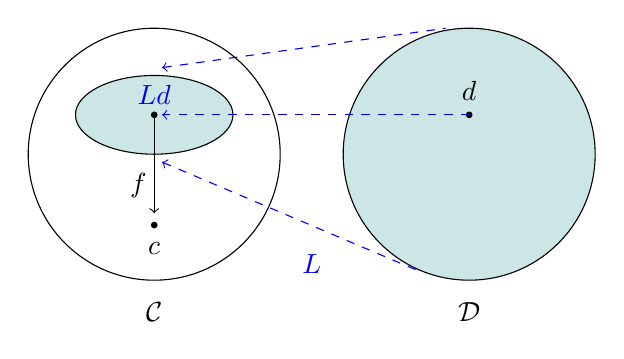
\begin{tikzpicture}
  \def\Xa{2.0};
  \def\Xb{-2.0};
  
  \def\Ytip{-0.9};
  \def\Yo{0.5}; % oval
  \def\Yb{-2.0}; % labels
         \draw (\Xa, 0)[fill=blue!50!green!20]  ellipse (1.6 and 1.6);
         \draw (\Xb , 0) ellipse (1.6 and 1.6);
         % oval
         \draw (\Xb , \Yo)[fill=blue!50!green!20] ellipse (1 and 0.5);
         
        % apex
        \filldraw (\Xb, \Ytip) circle (1pt);
        \node at ( \Xb, \Ytip - 0.3) { $c$ };
        
        % image
        \filldraw (\Xa, \Yo) circle (1pt);
        \node at ( \Xa, \Yo + 0.3) { $d$ };
        
	% middle of the cone
	\draw[->] (\Xb, \Yo) -- (\Xb, \Ytip + 0.15);
	\node at (\Xb - 0.2, \Ytip + 0.5) {$f$};
        	% sides of the cone
	%\draw (\Xb, \Ytip) -- (\Xb + 0.95, \Yo - 0.15);
	%\draw (\Xb, \Ytip) -- (\Xb - 0.95, \Yo - 0.15);

        % categories
        \node at (\Xa, \Yb) { $\mathcal D$ };
        \node at (\Xb, \Yb) { $\mathcal C$ };
        \node[blue] at (0, \Yb + 0.6) { $L$ };

        % functor middle
        \filldraw (\Xb, \Yo) circle (1pt);
        \node[blue] at ( \Xb, \Yo + 0.25) { $L d$ };
	\draw[->, blue, dashed] (\Xa, \Yo) -- (\Xb + 0.1, \Yo);
	% functor 
	\draw [<-, blue, dashed] (\Xb + 0.1, \Yo + 0.6)   --   (\Xa - 0.3, \Yo + 1.1);
	\draw [<-,blue, dashed] (\Xb + 0.1, \Yo - 0.6) -- (\Xa - 0.6, \Ytip - 0.6);
\end{tikzpicture}
\]



\texttt{comma 범주}\emph{comma 범주} $L/c$의 객체는 쌍 $\langle d, f \rangle$로, 여기서 $d$는 $\cat D$의 객체이고 $f \colon L d \to c$는 $\cat C$의 화살표입니다.

$\langle d, f \rangle$에서 $\langle d', f' \rangle$로 가는 사상(arrow)은 아래의 왼쪽 다이어그램을 가환하게 하는 사상 $h \colon d \to d'$입니다:
\[
 \begin{tikzcd}
 L d
 \arrow[rd, "f"']
 \arrow[rr, "L h"]
 && L d'
 \arrow[ld, "f'"]
 \\
 &c
  \end{tikzcd}
 \hspace{30pt}
\begin{tikzcd}
 d
 \arrow[rr, "h"]
 && d'
  \end{tikzcd}
\]

\subsection{Universal arrow}

$L$에서 $c$로 가는 유니버설 화살표는 콤마 카테고리 $L / c$에서 종말 대상으로 정의됩니다. 이 정의를 풀어보겠습니다. 종말 대상은 어떤 대상 $\langle d, f \rangle$에서 유일한 사상을 가지는 쌍 $\langle t, \tau \rangle$입니다. 이러한 사상은 다음의 교환 조건을 만족하는 화살표 $h \colon d \to t$입니다:
\[
 \begin{tikzcd}
 L d
 \arrow[rd, "f"']
 \arrow[rr, "L h"]
 && L t
 \arrow[ld, "\tau"]
 \\
 &c
  \end{tikzcd}
\]
즉, $\cat C (L d, c)$에 있는 모든 $f$에 대해 $\cat D (d, t)$에 있는 고유한 원소 $h$가 존재합니다. 여기서:
\[ f = \tau \circ L h \]
이러한 두 동형 사상의 원소 간의 일대일 대응은 기저의 부여론(adjunction) 을 암시합니다.

\subsection{Universal arrows from adjunctions}

먼저 함자 $L$이 오른쪽 수반 함자 $R$을 가질 때, 모든 $c$에 대해 $L$에서 $c$로의 보편 화살표(universal arrow)가 존재함을 자신에게 납득시켜 봅시다. 실제로, 이 화살표는 $\langle R c, \varepsilon_c \rangle$ 쌍에 의해 주어지며, 여기서 $\varepsilon$는 수반(adjunction)의 counit 입니다. 먼저, counit의 구성 요소는 콤마 카테고리 $L/c$의 객체에 대해 올바른 서명을 가지고 있습니다.
\[ \varepsilon_c \colon L (R c) \to c \]

$\langle R c, \varepsilon_c \rangle$가 $L/c$에서 말단 객체(terminal object)임을 보이고 싶습니다. 즉, 어떤 객체 $\langle d, f \colon L d \to c \rangle$에 대해서도 $f = \varepsilon_c \circ L h$를 만족하는 유일한 $h \colon d \to R c$가 존재합니다.
\[
 \begin{tikzcd}
 L d
 \arrow[rd, "f"']
 \arrow[rr, "L h"]
 && L (R c)
 \arrow[ld, "\varepsilon_c"]
 \\
 &c
  \end{tikzcd}
\]
이를 증명하기 위해, $\phi_{d c}$의 자연성 조건 중 하나를 $d$의 함수로 작성해 봅시다:
\[  \phi_{d c} \colon \mathcal{C} (L d, c) \to \mathcal{D}( d , R c)\]
어떠한 화살표 $h \colon d \to d'$에 대해서도 다음의 도형(diagram)이 가환(commute)해야 합니다:
\[
 \begin{tikzcd}
 \mathcal{C}(L d', c)
 \arrow[d, leftrightarrow, "\phi_{d', c}"]
 \arrow[r, "- \circ L h"]
 &
 \mathcal{C}(L d, c)
  \arrow[d, leftrightarrow, "\phi_{d, c}"]
 \\
 \mathcal{D}(d', R c)
 \arrow[r, "- \circ h"]
& \mathcal{D}(d, R c)
 \end{tikzcd}
\]
우리는 $d'$을 $R c$로 설정하여 Yoneda 트릭을 사용할 수 있습니.

\[
 \begin{tikzcd}
 \mathcal{C}(L (R c), c)
 \arrow[d, leftrightarrow, "\phi_{R c, c}"]
 \arrow[r, "- \circ L h"]
 &
 \mathcal{C}(L d, c)
  \arrow[d, leftrightarrow, "\phi_{d, c}"]
 \\
 \mathcal{D}(R c, R c)
 \arrow[r, "- \circ h"]
& \mathcal{D}(d, R c)
 \end{tikzcd}
\]
이제 우리는 hom-set $\cat D(R c, R c)$의 특수 요소, 즉 항등 화살표 $id_{R c}$를 선택하고 이를 다이어그램의 나머지 부분으로 전파할 수 있습니다. 왼쪽 위 모퉁이는 $\varepsilon_c$가 되고, 오른쪽 아래 모퉁이는 $h$가 되며, 오른쪽 위 모퉁이는 $h$의 adjoint(수반사)에 해당하는 $f$가 됩니다.

\[
 \begin{tikzcd}
\varepsilon_c
 \arrow[d, leftrightarrow, "\phi_{R c, c}"]
 \arrow[r, maps to, "- \circ L h"]
 &
f
  \arrow[d, leftrightarrow, "\phi_{d, c}"]
 \\
id_{R c}
 \arrow[r, maps to, "- \circ h"]
& h
 \end{tikzcd}
\]
위쪽 화살표는 우리가 추구하는 등식 $f = \varepsilon_c \circ L h$를 제공합니다.

\subsection{Adjunction from universal arrows}

반대의 결과는 더욱 흥미롭습니다. 만약 모든 $c$에 대해 $L$에서 $c$로의 유일한 화살이 존재해서 콤마 카테고리 $L/c$에서 종단 객체 $\langle t_c, \varepsilon_c \rangle$를 형성한다면, 우리는 $L$의 오른쪽 수반 함자(functor)인 $R$을 구성할 수 있습니다. 이 함자의 객체에 대한 동작은 $R c = t_c$로 주어지며, $\varepsilon_c$는 자동으로 $c$에 대해 자연스럽게 되고, 이는 수반의 공역(counit)을 형성합니다.

이중적 명제도 있습니 다: 상대성(Adjunction)은 $d/R$의 콤마 범주에서 초기 객체를 형성하는 유도 화살표 $\eta_d$의 집합에서 시작하여 구성할 수 있습니다.

이 결과들은 프레이드의 수반 함자 \textit{정리}(Freyd's adjoint functor theorem)를 증명하는 데 도움이 될 것~입니다.

\section{Properties of Adjunctions}

\subsection{Left adjoints preserve colimits}

여기서 극한(Colimit)은 보편(Universal) 쌍곡선(cocone)으로 정의되었~니다. 모든 쌍곡선---즉, 도형 $D \colon \cat J \to \cat C$에서 상수 함자(Constant Functor) $\Delta_x$로의 자연 변환---에 대해 유일한 분해 사상(Morphisms)이 극한 $\text{Colim}\, D$에서 $x$로 존재한~니다. 이 조건은 쌍곡선 집합과 동형 사상 집합(hom-set) 간의 일대일 대응으로 표현될 수 있~니다:
\[ [\cat J, \mathcal{C}](D, \Delta_x)  \cong \mathcal{C}( \text{Colim} \, D, x) \]
이 분해 조건은 이 동형사상의 자연성(naturality)에 의해 인코딩됩니다.

결국 동체(cones)의 집합, 그 자체로 $\Set$의 대상이 되는 집합은 다음과 같은 $\Set$ 값 함수자 $F \colon \cat J \to \Set$의 극한임이 밝혀졌습니다:
\[ F j = \cat C(D j, x) \]
이를 보여주기 위해, $F$의 극한(limit)에서 시작하여 코콘(cocones)의 집합으로 끝낼 것입니다. $\Set$ 값을 가지는 함자(functor)의 극한이 그 꼭짓점이 1(단일집합)인 원뿔(cones)의 집합과 같다는 것을 기억할 수 있을 것입니다. 우리 경우에는, 각각의 이러한 원뿔은 해당 호므셋(hom-set) $\cat C(D j, x)$로부터의 사상의 선택을 설명합니다:
\[
 \begin{tikzcd}
  & 1
\arrow[ddr, ""]
 \arrow[ddl, ""']
 \arrow[ddd, ""]
 \\
\\
\cat C( D j_1, x)
\arrow[rr, red]
\arrow[rd, red]
&& \cat C( D j_2, x)
\arrow[dl, red]
\\
& \cat C( D j_3, x)
 \end{tikzcd}
\]
이 각각의 사상들은 동일한 대상 $x$로의 목표를 가지므로, 이들은 꼭짓점 $x$를 가진 공모형(cocone)을 구성합니다.
\[
\begin{tikzcd}
 D j_1
 \arrow[rr, red]
 \arrow[dr, red]
 \arrow[dddr, ""']
 && D j_2
\arrow[dl, red]
 \arrow[dddl, ""]
 \\
 & D j_3
 \arrow[dd, ""]
 \\
 \\
 & x
 \end{tikzcd}
 \]
이 꼭지점이 $1$인 원뿔에 대한 가환 조건들은 동시에 이 꼭지점이 $x$인 공원뿔에 대한 가환 조건들입니다. 그러나 이것들은 정확히 집합 $[\cat J, \mathcal{C}](D, \Delta_x)$에서의 공원뿔들입니다.

따라서 원래의 코코넬 집합을 $\cat C (D-, x)$의 극한(limit)으로 대체할 수 있습니다:
\[ \text{Lim}\; \cat C (D-, x) \cong \cat C( \text{Colim}\,  D, x) \]
(반변 반함자(contravariant hom-functor))가 다이어그램 $D$에 작용한 극한은 이 다이어그램의 공극한에 작용한 반함자와 동형입니다. 이는 보통 다음과 같이 약칭됩니다: 반함자는 공극한을 보존합니다.

한글로 번역한 사한계를 보존하는 함자를 \index{co-continuous functor}공연속 함자(co-continuous)라고 합니다. 따라서 반변 공사함자(contravariant hom-functor)는 공연속 함자입니다.

이제 $L \colon \cat C \to \cat D$이고 $R$이 반대 방향으로 가는 adjunction $L \dashv R$이 있다고 가정합니다. 좌측 함수자 $L$이 colimit를 보존함을 보이고자 합니다, 즉:
\[ L (\text{Colim} \, D) \cong \text{Colim} (L \circ D) \]
어떤 다이어그램 $D \colon \cat J \to \cat C$의 콜리밋이 존재한다고 가정합니다.

\textbf{요네다 보조정리}를 사용하여 임의의 $x$에 대한 양쪽에서 나오는 사상이 동형임을 보여줍니다:
\[ \cat D( L (\text{Colim} \, D), x) \cong \cat D (\text{Colim} (L \circ D), x) \]
왼쪽 면에 adjunction을 적용하여 얻습니다:
\[ \cat D( L (\text{Colim} \, D), x) \cong \cat C (\text{Colim}\, D, R x) \]
쌍대함자에 의한 쌍대극한의 보존은 다음과 같은 결과를 줍니다:
\[ \cong \text{Lim}\; \cat C(D -, R x) \]
또한 adjunction(쌍대) 을 사용하여, 우리는 다음과 같은 결과를 얻습니다:
\[ \cong \text{Lim}\; \cat D((L \circ D) -, x) \]
그리고 콜리밋(colimits) 보존의 두 번째 응용은 우리에게 원하는 결과를 제공합니다:
\[ \cong  \cat D((\text{Colim}\;(L \circ D), x) \]

이 결과를 사용하여 데카르트 닫힌 범주에서의 분배법칙에 대한 이전 증명을 재구성할 수 있습니. 우리는 곱(product)가 지수(exponential)의 왼쪽 수반함수(left adjoint)임을 이용합니. 왼쪽 수반함수는 쌍극한(colimit)을 보존합니. 쌍대곱(coproduct)은 쌍극한이므로, 따라서:
\[(b + c) \times a \cong b \times a + c \times a \]
여기서 왼쪽 함자(functor)는 $L x = x \times a$이며, 다이어그램(diagram) $D$는 객체(object) $b$와 $c$의 쌍을 선택합니다.

\subsection{Right adjoints preserve limits}
이중 논증을 사용하면, 오른쪽 수반 함자들(right adjoints)은 극한(limits)을 보존한다는 것을 보일 수 있습니다, 즉:
\[ R (\text{Lim}\, D) \cong \text{Lim}\, (R \circ D) \]

우리는 (공변) hom-함수가 극한을 보존함을 보여주는 것으로 시작합니다.
\[ \text{Lim}\; \cat C( x, D-) \cong \mathcal{C}(x, \text{Lim}\,D) \]
이는 한계(limits)를 정의하는 원뿔의 집합이 $\Set$-값 함수자(functor)의 한계와 동형(isomorphic)임을 나타내는 주장에서 따릅니다:
\[ F j = \cat C(x, D j) \]
한계를 보존하는 함자를 \index{continuous functor} 계속적 함자라고 합니다.

$L \dashv R$의 부여(adjunction)가 주어졌을 때, 오른쪽 함자 $R \colon \cat D \to \cat C$가 극한(limits)을 보존함을 보이기 위해, 우리는 요네다(Yoneda) 주장을 사용합니다:
\[ \cat C(x, R (\text{Lim}\, D)) \cong \cat C (x, \text{Lim}\, (R \circ D)) \]
확실히, 우리는 다음과 같습니다:
\[ \cat C(x, R (\text{Lim}\, D)) \cong \cat D(L x, \text{Lim}\, D) \cong \text{Lim}\; \cat D(L x, D-) \cong \cat C(x, \text{Lim}\, (R \circ D))\]


\section{Freyd의 수반 함자 정리}

일반적으로 함자들(함수자들)은 정보를 잃기 쉽습니다---즉, 역함자(역함수자)가 존재하지 않습니다. 일부 경우에는 잃어버린 정보를 ``최적의 추정치(best guess)''로 대체함으로써 보완할 수 있습니다. 이를 체계적으로 수행하면, 수반(adjunction) 관계가 됩니다. 문제는: 두 카테고리(범주) 사이의 함자(함수자)가 주어졌을 때, 수반 함자(함수자)를 구성할 수 있는 조건은 무엇인가입니다.

이 질문에 대한 대답은 Freyd의 수반 함수 정리(adjoint functor theorem)에 의해 주어집니다. 처음에는 이것이 해 집합 조건(solution set condition)이라는 매우 추상적인 구성과 관련된 기술적 정리처럼 보일 수 있습니다. 나중에 이 조건이 함수 제거(defunctionalization)라는 프로그래밍 기법으로 직접 변환됨을 볼 것입니다.

이어서, 함수자 $L \colon \cat D \to \cat C$의 오른쪽 수반 함수를 구성하는 데 주의를 기울일 것입니다. 반대 문제를 해결하기 위해서는 함수자 $R \colon \cat C \to \cat D$의 왼쪽 수반 함수를 찾는 이중 논리를 사용할 수 있습니.

첫 번째 관찰은, 부여된 편함수(adjunction)에서 왼쪽 함자(함수자)가 쌍극한(colimit)을 보존하기 때문에, 우리의 함자 $L$이 쌍극한을 보존해야 한다는 점입니다. 이는 오른쪽 수반 함자를 구성하는 것이 $\cat D$에서 쌍극한을 구성할 수 있는 능력에 의존하며, 이들을 $L$을 사용하여 어떻게든 $\cat C$로 다시 옮길 수 있는 능력에도 의존한다는 힌트를 제공합니다.

모든 쌍대극한(colimits), 큰 것과 작은 것이 $\cat{D}$에 존재한다고 요구할 수 있지만, 이 조건은 너무 강합니다. 모든 쌍대극한을 가지는 작은 카테고리는 자동적으로 전순서(preorder)여야 합니다---즉, 두 객체 사이에 하나 이상의 사상이 존재할 수 없습니다.

하지만 잠시 크기 문제를 무시하고, 소스 범주 \(\cat D\)가 작고 모든 쌍극한(colimit)을 가지는(따라서 전순서(preorder)입니다) 쌍극한 보존 함자 \(L\)의 오른쪽 수반 함자가 어떻게 구성되는지 살펴봅시다.

\subsection{Freyd의 정리(Freyd's theorem) in a preorder}

$L$의 우측 수반(functor)(right adjoint)을 정의하는 가장 쉬운 방법은, 모든 객체 $c$에 대해 $L$에서 $c$로 가는 보편적인 화살표(universal arrow)를 구성하는 것입니다. 이러한 화살표는 콤마 카테고리(comma category) $L/c$—즉 $L$의 이미지에서 시작하여 객체 $c$에 도달하는 화살표들의 카테고리—에서의 종단 객체(terminal object)입니다.

\[
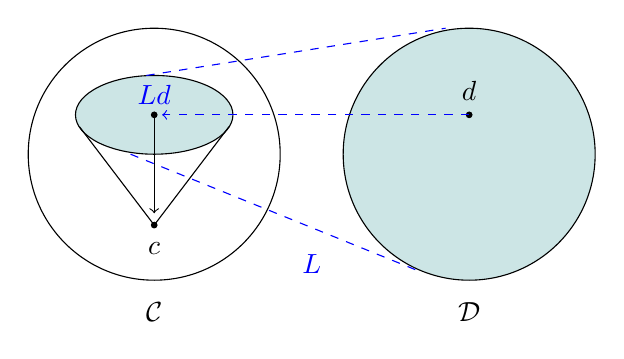
\begin{tikzpicture}
  \def\Xa{2.0};
  \def\Xb{-2.0};
  
  \def\Ytip{-0.9};
  \def\Yo{0.5}; % oval
  \def\Yb{-2.0}; % labels
         \draw (\Xa, 0)[fill=blue!50!green!20]  ellipse (1.6 and 1.6);
         \draw (\Xb , 0) ellipse (1.6 and 1.6);
         % oval
         \draw (\Xb , \Yo)[fill=blue!50!green!20] ellipse (1 and 0.5);
         
        % apex
        \filldraw (\Xb, \Ytip) circle (1pt);
        \node at ( \Xb, \Ytip - 0.3) { $c$ };
        
        % image
        \filldraw (\Xa, \Yo) circle (1pt);
        \node at ( \Xa, \Yo + 0.3) { $d$ };
        
	% middle of the cone
	\draw[->] (\Xb, \Yo) -- (\Xb, \Ytip + 0.15);
        	% sides of the cone
	\draw (\Xb, \Ytip) -- (\Xb + 0.95, \Yo - 0.15);
	\draw (\Xb, \Ytip) -- (\Xb - 0.95, \Yo - 0.15);

        % categories
        \node at (\Xa, \Yb) { $\mathcal D$ };
        \node at (\Xb, \Yb) { $\mathcal C$ };
        \node[blue] at (0, \Yb + 0.6) { $L$ };

        % functor middle
        \filldraw (\Xb, \Yo) circle (1pt);
        \node[blue] at ( \Xb, \Yo + 0.25) { $L d$ };
	\draw[->, blue, dashed] (\Xa, \Yo) -- (\Xb + 0.1, \Yo);
	% functor 
	\draw [blue, dashed] (\Xb - 0.1, \Yo + 0.5    )   --   (\Xa - 0.3, \Yo + 1.1);
	\draw [blue, dashed] (\Xb - 0.3, \Yo - 0.5) -- (\Xa - 0.6, \Ytip - 0.6);
\end{tikzpicture}
\]

중요한 관찰은 이 쉼표 범주가 $\cat C$에서의 쌍대원뿔(cocone)을 설명한다는 것입니다. 이 쌍대원뿔의 바탕(base)은 $c$를 방해 없이 볼 수 있는 $L$의 이미지에 있는 대상들로 형성됩니다. 쌍대원뿔의 바탕에 있는 화살표들은 $L/c$의 사상(morphisms)들입니다. 이들은 쌍대원뿔의 측면을 가환하게 만드는 화살표들입니다.
\[
 \begin{tikzcd}
 L d
 \arrow[rd, "f"']
 \arrow[rr, "L h"]
 && L d'
 \arrow[ld, "f'"]
 \\
 &c
  \end{tikzcd}
 \hspace{30pt}
\begin{tikzcd}
 d
 \arrow[rr, "h"]
 && d'
  \end{tikzcd}
\]

이 꼬콘의 기초(base)는 $\cat D$로 다시 투영될 수 있습니 다. 모든 쌍 $(d, f)$을 $L/c$에서 $d$로 되돌리는 투영 $\pi_c$가 있습니 다. 이 투영은 화살표 $f$를 무시합니 다. 또한 $L/c$의 모든 사상(morphism)을 $\cat D$에서 비롯된 화살표로 사상합니 다. 이러한 방법으로 $\pi_c$는 $\cat D$에서 다이어그램(diagram)을 정의합니 다. 이 다이어그램의 콜리밋(colimit)이 존재하는데, 이는 우리가 $\cat D$에서 모든 콜리밋이 존재한다고 가정했기 때문입니 다. 이 콜리밋을 $t_c$라고 부르겠습니 다.
\[ t_c = \text{colim}\; \pi_c \]

\[
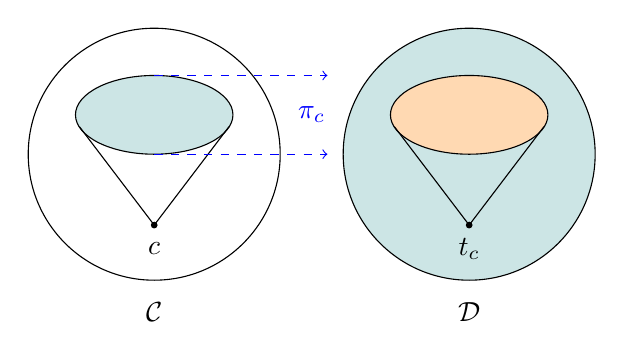
\begin{tikzpicture}
  \def\Xa{2.0};
  \def\Xb{-2.0};
  
  \def\Ytip{-0.9};
  \def\Yo{0.5}; % oval
  \def\Yb{-2.0}; % labels
         \draw (\Xa, 0)[fill=blue!50!green!20]   ellipse (1.6 and 1.6);
         \draw (\Xb , 0) ellipse (1.6 and 1.6);
         % oval
         \draw (\Xb , \Yo)[fill=blue!50!green!20]  ellipse (1 and 0.5);

        % apex
        \filldraw (\Xb, \Ytip) circle (1pt);
        \node at ( \Xb, \Ytip - 0.3) { $c$ };
                
        	% sides of the cone
	\draw (\Xb, \Ytip) -- (\Xb + 0.95, \Yo - 0.15);
	\draw (\Xb, \Ytip) -- (\Xb - 0.95, \Yo - 0.15);

         % second oval
         \draw (\Xa , \Yo) [fill=orange!30]  ellipse (1 and 0.5);
          
        % apex
        \filldraw (\Xa, \Ytip) circle (1pt);
        \node at ( \Xa, \Ytip - 0.3) { $t_c$ };

        	% sides of the cone
	\draw (\Xa, \Ytip) -- (\Xa + 0.95, \Yo - 0.15);
	\draw (\Xa, \Ytip) -- (\Xa - 0.95, \Yo - 0.15);

        % categories
        \node at (\Xa, \Yb) { $\mathcal D$ };
        \node at (\Xb, \Yb) { $\mathcal C$ };
        \node[blue] at (0, \Yo) { $\pi_c$ };

	% functor 
	\draw [->, blue, dashed] (\Xb, \Yo + 0.5) --  (\Xb + 2.2, \Yo + 0.5);
	\draw [->, blue, dashed] (\Xb, \Yo - 0.5)  -- (\Xb + 2.2, \Yo - 0.5);
\end{tikzpicture}
\]

현재 이 $t_c$를 이용하여 $L/c$에서 끝 대상(terminal object)을 구성할 수 있는지 살펴봅시다. 화살표 하나를 찾아야 합니다. 이를 $\varepsilon_c \colon L t_c \to c$라고 부릅시다. 이 쌍 $\langle t_c, \varepsilon_c \rangle$가 $L/c$에서 끝 대상이 되도록 해야 합니다.

$L$이 $\pi_c$에 의해 생성된 다이어그램을 $L/c$에 의해 정의된 코콘의 base(기저)로 다시 매핑함을 주목하세요. 투영 $\pi_c$는 이 코콘의 면을 무시하고 기저를 그대로 두는 것 외에는 아무것도 하지 않았습니다.

이제 우리는 동일한 기저(base)를 가진 두 개의 코콘(cocone)을 범주 $\cat C$에서 가지고 있습니니다: 정점(apex) $c$를 가진 원래의 코콘과 범주 $\cat D$의 코콘에 $L$을 적용하여 얻은 새로운 코콘입니다. $L$이 쳅극(limits)을 보존(bepreserve)하므로, 새로운 코콘의 쳅극은 $L t_c$---쳅극 $t_c$의 이미지(image)입니다:

\[ \text{colim} \; (L \circ \pi_c) = L ( \text{colim} \; \pi_c) = L t_c\]

범용적 구성(universal construction)에 의해, 우리는 유일한 코원뿔 사상(cocone morphism)이 귀한 $L t_c$에서 $c$로 존재해야 한다는 것을 추론합니다. 그 사상을 $\varepsilon_c$라 부르기로 하며, 이 사상은 관련된 삼각형들을 교환(commute)하게 만듭니다.

보여야 할 남은 것은 $\langle t_c, \varepsilon_c \rangle$가 $L/c$에서 \emph{종단객체}(terminal object)임입니다. 즉, 임의의 $\langle d, f \colon L d \to c \rangle$에 대해, 다음 삼각형을 가환하도록 만드는 유일한 콤마-범주 사상(comma-category morphism) $h \colon d \to t_c$가 존재함을 보이는 것입니다:

\[
 \begin{tikzcd}
 L d
 \arrow[rd, "f"']
 \arrow[rr, "L h"]
 && L t_c
 \arrow[ld, "\varepsilon_c"]
 \\
 &c
  \end{tikzcd}
\]

이러한 $d$는 자동으로 $\pi_c$에 의해 생성된 다이어그램의 일부가 됩니다 ($\langle d, f \rangle$에 $\pi_c$가 작용한 결과입니다). 우리는 $t_c$가 이 다이어그램의 극한이라는 것을 알고 있습니다. 따라서 극한 공원뿔(limiting cocone)에서 $d$에서 $t_c$로 가는 와이어가 존재해야 합니다. 우리는 이 와이어를 우리의 $h$로 선택합니다.

\[
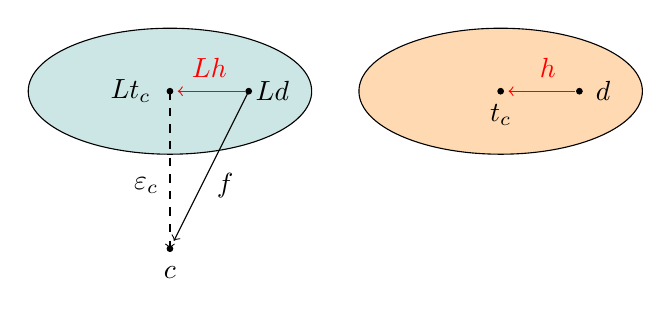
\begin{tikzpicture}
  \def\Xa{2.1};
  \def\Xb{-2.1};
  
  \def\Ytip{0};
  \def\Ybot{-2};
  \def\Yo{0}; % oval
  \def\Yf{-1.2}; % label
         % first oval
         \draw (\Xb , \Yo)[fill=blue!50!green!20]  ellipse (1.8 and 0.8);

         % second oval
         \draw (\Xa , \Yo) [fill=orange!30]  ellipse (1.8 and 0.8);
          
        % apex L tc
        \filldraw (\Xb, \Ytip) circle (1pt);
        \node at ( \Xb - 0.5, \Ytip) { $L t_c$ };
        
        % apex c
        \filldraw (\Xb, \Ybot) circle (1pt);
        \node at ( \Xb, \Ybot - 0.3) { $c$ };
                
        	% sides of the cone L h
	\draw[red, ->]  (\Xb + 0.95, \Yo) -- (\Xb + 0.1, \Ytip);
	\node[red] at (\Xb + 0.5, \Ytip + 0.3) {$L h$};

        % apex tc
        \filldraw (\Xa, \Ytip) circle (1pt);
        \node at ( \Xa, \Ytip - 0.3) { $t_c$ };

        	% sides of the cone h
	\draw [->, red] (\Xa + 0.95, \Yo) -- (\Xa + 0.1, \Ytip);
	\node[red] at ( \Xa + 0.6, \Ytip + 0.3) { $h$ };
	
	% d
        \filldraw (\Xa + 1, \Yo) circle (1pt);
        \node at ( \Xa + 1.3, \Yo) { $d$ };

	% L d
        \filldraw (\Xb + 1, \Yo) circle (1pt);
        \node at ( \Xb + 1.3, \Yo) { $L d$ };
        
        % f
        \draw[->] (\Xb + 1, \Yo) to (\Xb + 0.05, \Ybot + 0.1);
        \node at (\Xb + 0.7, \Yf) {$f$};
        
        % epsilon
        \draw[->, dashed] (\Xb, \Ytip) -- (\Xb, \Ybot);
        \node at (\Xb - 0.3, \Yf) {$\varepsilon_c$};

\end{tikzpicture}
\]
순환 조건은 $\varepsilon_c$가 공원 사상(cocone morphism)이기 때문에 따릅니다. $\cat D$가 사전순서(preorder)이기 때문에 그러한 사상은 유일합니다.

이는 모든 $c$에 대해 유일성 화살표(universal arrow) $\langle t_c, \varepsilon_c \rangle$가 있음을 증명합니다. 따라서 우리는 객체에 대해 $R c = t_c$로 정의된 함자(functor) $R$을 가지며, 이는 $L$의 오른쪽 수반 함자(right adjoint)입니다.

\subsection{Solution set condition}

이전 증명의 문제는 쉼표 범주(comma categories)가 대부분의 실제 상황에서 크다는 것~입니다: 그들의 객체들이 집합을 형성하지 않습니다. 그러나 아마도 우리는 더 작지만 대표적인 객체와 화살들의 집합을 선택함으로써 쉼표 범주를 근사할 수 있을~지도 모릅니다.

어떤 색인 집합 $I$에서 객체를 선택하기 위해 사상을 사용합니다. 객체들의 집합 $d_i$를 정의합니다, 여기서 $i \in I$입니다. 우리가 comma category $L/c$를 근사하려고 하기 때문에, 객체들을 화살표 $f_i \colon L d_i \to c$와 함께 선택합니다.

콤마 범주(comma category)의 관련 부분은 교환 조건(commuting condition)을 만족하는 객체(object)들 사이의 사상(morphism)으로 인코딩되었습니다. 이 조건을 우리의 객체 집합 내부에만 적용하도록 특수화하는 것을 시도할 수 있지만, 그 정도로는 충분하지 않 ~습니다. 우리는 콤마 범주의 모든 다른 객체들을 조사할 방법을 찾아야 합니다.

이를 위해, 우리는 임의의 $f \colon L d \to c$를 쌍 $\langle d_i, f_i \rangle$을 통해 분해하는 방법으로 교환 조건을 재해석합니다:
\[
 \begin{tikzcd}
 L d
 \arrow[rd, "f"']
 \arrow[rr, "L h"]
 && \textcolor{red}{L d_i}
 \arrow[ld, red, "f_i"]
 \\
 &c
  \end{tikzcd}
\]

A \index{해결 집합}\emph{해결 집합(solution set)}은 집합 $I$에 의해 인덱스된 쌍 $\langle d_i, f_i \colon L d_i \to c \rangle $의 모임으로, 이는 임의의 쌍 $\langle d, f \colon L d \to c \rangle $를 분해하는 데 사용될 수 있습니. 이는 인덱스 $i \in I$와 $f$를 분해하는 화살표 $h \colon d \to d_i$가 존재함을 의미합니다:
\[ f = f_i \circ L h \]

이 속성을 표현하는 또 다른 방법은 콤마 범주 $L/c$에서 \index{약 단말 집합}\emph{약 단말} 객체 집합이 존재한다고 말하는 것입니다. 약 단말 집합은 범주의 어떤 객체에 대해서도 그 집합에 속한 적어도 하나의 객체로 가는 사상이 존재하는 성질을 갖습니다.

이전에는 모든 $c$에 대해 comma 범주 $L/c$에서 종륙 객체(terminal object)를 갖는 것이 adjunction을 정의하기에 충분하다는 것을 보았습니다. 해결 집합(solution set)을 사용하여 동일한 목표를 달성할 수 있다는 것이 밝혀졌습니다.

Freyd의 수반 함자 정리의 가정은 작은 쌍대 완비 범주 $\cat D$에서 $\cat C$로의 귀한을 보존하는 함자(functor) $L \colon \cat D \to \cat C$가 있음을 명시합니다. 이 두 조건은 \emph{작은} 도형(diagram)과 관련이 있습니다. 만약 모든 $c$에 대해 해결 집합(solution set) $\langle d_i, f_i \colon L d_i \to c \rangle $을 선택할 수 있다면, 오른쪽 수반 함자(right adjoint) $R$이 존재합니다. 다양한 $c$에 대한 해결 집합들은 서로 다를 수 있습니다.

우리는 이미 쌍대완비 범주(cocomplete category)에서 약한 끝 대상(weakly terminal set)의 존재가 종말 대상(terminal object)을 정의하기에 충분하다는 것을 보았습니다. 우리의 경우, 임의의 $c$에 대해 $L$에서 $c$로 가는 보편 화살표(universal arrow)를 구성할 수 있다는 것을 의미합니다. 그리고 이것만으로 전체 부수 함자(adjunction)를 정의하기에 충분합니다.

부수 함자 정리(adjoint functor theorem)의 쌍대 버전은 왼쪽 부수 함자를 구성하는 데 사용할 수 있습니다.

\subsection{Defunctionalization}

모든 프로그래밍 언어는 함수를 정의할 수 있게 해줍니다, 하지만 모든 언어가 고급 함수(함수를 인수로 받거나 함수를 반환하는 함수)나 익명 함수(일명 람다)를 지원하지는 않습니다. 심지어 그런 언어들에서도 고차 함수는 디펑셔널화(defunctionalization)라는 과정을 통해 구현될 수 있습니다. 이 기법은 부속 함자 정리(adjoint functor theorem)에 기초합니다. 더욱이, 디펑셔널화는 예를 들어 분산 시스템과 같이 함수를 전달하는 것이 실용적이지 않을 때 사용할 수 있습니다.

디펑셔널라이제이션(defunctionalization) 뒤에 있는 아이디어는 함수 타입이 곱(product)의 오른쪽 수반자(right adjoint)로 정의된다는 것입니다.
\[ \cat C(e \times a, b) \cong \cat C(e, b^a) \]
좌수 준수성 정리(Adjoint functor theorem)은 이 보조 함자(adjoint)를 근사하는 데 사용할 수 있습니다.

일반적으로, 유한한 프로그램은 오직 유한한 수의 함수 정의만 가질 수 있습니니다. 이러한 함수(그리고 그것들이 캡처하는 환경들)는 우리가 함수 타입을 구성할 때 사용할 수 있는 해 집합을 형성합니다. 실제로, 우리는 다른 함수에 대한 인자로 나타나거나, 다른 함수로부터 반환되는 작은 부분 집합의 함수들에 대해서만 그것을 수행합니다.

고차 함수의 사용 예로 전형적인 것은 연속 전달 방식(Continuation Passing Style)입니다. 예를 들어, 이는 리스트의 요소들의 합을 계산하는 함수입니다. 하지만 합을 반환하는 대신에 연속 \hask{k}을 호출합니다:
\begin{haskell}
sumK :: [Int] -> (Int -> r) -> r
sumK [] k = k 0
sumK (i : is) k =
  sumK is (\s -> k (i + s))
\end{haskell}
목록이 비어 있으면 함수는 계속 함수(continuation)를 0과 함께 호출합니다. 그렇지 않으면 두 개의 인수를 사용하여 자신을 재귀적으로 호출합니다: 목록의 꼬리 \hask{is}, 그리고 새로운 계속 함수(continuation):
\begin{haskell}
\s -> k (i + s)
\end{haskell}
이 새로운 연속(continuation)은 이전 연속 \hask{k}를 호출하면서 리스트의 첫 요소와 그 인자 \hask{s} (즉, 누적 합)을 더한 값을 전달합니다.

이 람다(lambda)를 클로저(closure)라고 하는 이유를 주목하십시오: 이는 하나의 변수 \hask{s}의 함수지만, 그 환경에서 \hask{k} 및 \hask{i}에도 접근할 수 있습니다.

최종 합계를 추출하기 위해 우리는 자명한 연속(continuation), 항등 함수를 사용하여 재귀 함수(recursive function)를 호출합니다:
\begin{haskell}
sumList :: [Int] -> Int
sumList as = sumK as (\i -> i)
\end{haskell}

익명 함수는 편리하나, 명명된 함수를 사용하는 것을 막는 것은 없습다. 그러나, 만약 후속 작업을 분리하고자 한다면, 환경을 전달하는 것에 대해 명확하게 해야 합니다.

예를 들어, 우리는 첫 번째 람다를 함수 \hask{more}로 대체할 수 있지만, 타입 \hask{(Int, Int -> r)}의 환경을 명시적으로 전달해야 합니다.
\begin{haskell}
more :: (Int, Int -> r) -> Int -> r
more (i, k) s = k (i + s)
\end{haskell}
다른 람다(λ), 즉 항등함수(identity)는 빈 환경을 사용합니다:
\begin{haskell}
done :: Int -> Int
done i = i
\end{haskell}
다음은 명명된 함수들을 사용한 우리의 알고리즘 구현입니다:
\begin{haskell}
sumK' :: [Int] -> (Int -> r) -> r
sumK' [] k = k 0
sumK' (i : is) k =
  sumK' is (more (i, k))
\end{haskell}

\begin{haskell}
sumList :: [Int] -> Int
sumList is = sumK' is done
\end{haskell}

사실 우리가 관심 있는 것이 합계를 계산하는 것이라면, 다형성 타입 \hask{r}를 \hask{Int}로 바꾸고 다른 변경은 하지 않아도 됩니다.

이 구현은 여전히 고차 함수를 사용합니다. 이를 없애기 위해, 함수를 인수로 전달하는 것이 무엇을 의미하는지 분석해야 합니다. 그런 함수는 오직 한 가지 방식으로만 사용할 수 있습니다: 인수에 적용될 수 있습니다. 함수 타입의 이러한 특성은 커링(kKurrying) 조합의 counit으로 표현됩니다:
\[ \varepsilon \colon b^a \times a \to b \]
또는, Haskell에서처럼, 고차 함수(higher-order function)로:
\begin{haskell}
apply :: (a -> b, a) -> b
\end{haskell}
이번에는 초항(훔초항, counit)을 기본 원리부터 구성하는 데 관심이 있습니다. 우리는 쉼표 범주(comma category)를 사용하여 이를 달성할 수 있다는 것을 보았습니다. 우리의 경우, 곱 함자 $L_a = (-) \times a$의 쉼표 범주의 객체는 쌍입니다.
\[(e, f \colon (e \times a) \to b) \]
혹은, Haskell에서:
\begin{haskell}
data Comma a b e = Comma e ((e, a) -> b)
\end{haskell}
이 범주에서 $(e, f)$와 $(e', f')$ 사이의 사상(morphism)은 $e \to e'$로 가는 화살표(arrow) $h$이며, 다음의 교환 조건을 만족합니다:
\[ f' \circ h = f \]
우리는 이 사상을 환경을 ``축소하는'' 것으로 해석합니다. 화살표 $f'$는 $h(e)$로 주어진 잠재적으로 더 작은 환경을 사용하여 동일한 유형 $b$의 출력을 생성할 수 있습니다. 예를 들어 $e$는 $a$로부터 $b$를 계산하는 데 관련 없는 변수를 포함할 수 있으며, $h$는 해당 변수들을 제외합니다.

사실, 우리는 \hask{more}와 \hask{done}을 정의할 때 이러한 종류의 축소를 수행했습니. 원칙적으로, 우리는 \hask{is}를 두 함수에 모두 전달할 수 있었습니, 왜냐하면 호출 시점에서 접근할 수 있기 때문입니다. 하지만 그들이 그것을 필요로 하지 않는다는 것을 알고 있습니다.

형식적으로, 우리는 함수 객체 $a \to b$를 코마 범주에 의해 정의된 도표의 콜리밋(colimit)으로 정의할 수 있습니니다. 이러한 콜리밋은 본질적으로 코마 범주 사상(comma-category morphisms)에 의해 주어진 동일시로 표현된 모든 환경의 거대한 쌍대곱(coproduct)입니다. 이러한 동일시는 $a \to b$가 필요한 환경을 최소한으로 줄이는 역할을 합니다.

우리의 예제에서, 우리가 관심 있는 연속 함수들은 함수 \hask{Int -> Int}입니다. 사실 우리는 일반적인 함수 유형 \hask{Int -> Int}을 생성하는 데 관심이 있는 것이 아니라 \hask{more}와 \hask{done}이라는 두 함수를 수용할 수 있는 최소한의 함수 유형에만 관심이 있습니다. 이를 통해 매우 작은 해집합을 생성하여 해결할 수 있습니다.

우리의 경우 해집합은 $(e_i, f_i \colon L_a e_i \to b)$의 쌍으로 구성되어 있으며, 어떤 쌍 $(e, f \colon L_a e \to b)$도 $f_i$ 중 하나를 통해 인수분해될 수 있는 한입니다. 더 정확히 말하자면, 우리가 관심 있는 두 환경은 \hask{(Int, Int ->Int)}로 \hask{more}에 해당하고, 빈 환경 \hask{()}로 \hask{done}에 해당합니다.

원칙적으로, 우리의 해 집합은 콤마 카테고리의 모든 객체들을 다음과 같은 형태의 쌍으로 분해할 수 있어야 합니다:
\begin{haskell}
(e, (e, Int) -> Int)
\end{haskell}
하지만 여기서는 두 가지 특정한 함수들에만 관심이 있습니. 또한 표현의 유일성에 대해서는 신경 쓰지 않기 때문에, (어울림 함자 정리에서 했던 것처럼) 공극(limit)를 사용하지 않고, 관심 있는 모든 환경의 쌍대곱(coproduct)을 사용할 것입니다. 그 결과 우리는 우리가 관심 있는 두 환경의 합집합인 다음과 같은 데이터 타입을 얻게 됩니다:
\begin{haskell}
data Kont = Done | More Int Kont
\end{haskell}
우리가 \hask{Int -> Int} 환경의 일부(우리가 \hask{more}에 사용했던 부분)를 \hask{Kont}로 재귀적으로 인코딩한 것을 주목하십시오.

이 정의를 자세히 살펴보면, 몇 가지 이름만 바뀐 \hask{Int} 목록의 정의라는 것을 알 수 있을 것입니다. \hask{More}에 대한 모든 호출은 \hask{Kont} 스택에 또 다른 정수를 푸시(push)합니다. 이 해석은 재귀 알고리즘이 어떤 형태로든 런타임 스택을 필요로 한다는 우리의 직관과 일치합니다.

이제 adjunction의 counit에 대한 우리의 근삿값을 구현할 준비가 되었습니다. 이는 두 함수의 본체로 구성되며, 재귀 호출도 \hask{apply}를 거친다는 이해를 바탕으로 합니다.
\begin{haskell}
apply :: (Kont, Int) -> Int
apply (Done, i) = i
apply (More i k, s) = apply (k, i + s)
\end{haskell}
주요 알고리즘을 이제 고차 함수나 람다 없이 다시 작성할 수 있습니:
\begin{haskell}
sumK'' :: [Int] -> Kont -> Int
sumK'' [] k = apply (k, 0)
sumK'' (i : is) k = sumK'' is (More i k)
\end{haskell}

\begin{haskell}
sumList'' is = sumK'' is Done
\end{haskell}

융역활(literal translation)화(defunctionalization)의 주요 장점은 분산 환경에서도 사용할 수 있다는 점입니다. 원격 함수의 인자가 데이터 구조이고 함수가 아닌 경우, 이를 직렬화(serialize)하여 전송할 수 있습니다. 수신자가 \hask{apply}에 접근할 수 있으면 됩니다.

\section{자유/망각 수반(Functor) 관계}
Adjunction에서 두 functor는 서로 다른 역할을 합니다: adjunction의 그림은 대칭적이지 않습니다. 이는 자유/망각 adjunctions의 경우에서 가장 잘 설명됩니다.

망각 함자(미국어: forgetful functor)는 원천 범주에서 일부 구조를 "망각"하는 함자(영문 용어: functor)입니다. 이는 엄격한 정의는 아니지만, 대부분의 경우 무엇이 망각되는 구조인지 명확합니다. 매우 자주 목적 범주는 구조가 없다고 간주되는 집합의 범주(영문 용어: category of sets)가 됩니다. 그 경우 망각 함자의 결과는 "기본" 집합(영문 용어: underlying set)이라고 불리며, 함자 자체는 종종 $U$라고 불립니다.

보다 정확하게, 우리는 한 함자가 \emph{구조}(structure)를 잊어버린다고 말합니다. 만약 hom-집합의 사상이 전사(mapping of hom-sets is not surjective)하지 않다면, 다시 말해, 대상 hom-집합에는 근원 hom-집합에 해당하는 사상들이 없는 사상들이 존재한다면 그렇습니다. 직관적으로, 이것은 근원에 있는 사상들이 유지해야 하는 어떤 구조(structure)를 가지고 있기 때문에 그 수가 적다는 것을 의미하며, 그 구조가 대상에는 없다는 것을 의미합니다.

잊어버리는 함자(Forgetful functor)에 대한 왼쪽 수반 함자(adjoint functor)를 \emph{자유 함자}(free functor)라고 부릅니다.

\[
 \begin{tikzcd}
F x
\arrow[d, bend right, red, dashed]
\arrow[d, dashed]
\arrow[d, bend left, blue, dashed]
  &&
  x
\arrow[d, bend right, red, dashed]
\arrow[d, dashed]
\arrow[d, bend left, blue, dashed]
 \arrow[ll, bend right, "F"']
 \\
y
   \arrow[rr, bend right, "U"']
 &&
 U y
  \end{tikzcd}
\]

자유/망각 adjunction(부착)의 고전적인 예는 자유 모노이드(free monoid)의 구성입니다.


\subsection{The category of monoids}
모노이드(monoid) 단일 범주 $\mathcal{C}$에서 모노이드들은 그들 자체의 범주 $\mathbf{Mon}(\mathcal{C})$를 형성합니다. 그 객체들은 모노이드들이고, 그 화살표들은 모노이드 구조를 보존하는 $\mathcal{C}$ 내의 화살표들입니다.

다음 다이어그램은 $f$가 모노이드 사상(monoid morphism)이라는 것이 무엇을 의미하는지 설명하며, 모노이드 $(M_1, \eta_1, \mu_1)$에서 모노이드 $(M_2, \eta_2, \mu_2)$로 가는 과정을 보여 줍니다:
\[
 \begin{tikzcd}
 & M_1
 \arrow[dd, "f"]
 & M_1 \otimes M_1
 \arrow[l, "\mu_1"]
 \arrow[dd, "f \otimes f"]
 \\
 I
 \arrow[ru, "\eta_1"]
 \arrow[rd, "\eta_2"']
 \\
 & M_2
 & M_2 \otimes M_2
 \arrow[l, "\mu_2"]
  \end{tikzcd}
\]
모노이드 사상 $f$는 단위원을 단위원으로 사상해야 하며, 이는 다음을 의미합니다:
\[ f \circ \eta_1 = \eta_2 \]
곱셈을 곱셈에 매핑해야 합니다.
\[ f \circ \mu_1 = \mu_2 \circ (f \otimes f)\]
기억하세요, 텐서곱 $\otimes$는 함자적(funtorial)입니다, 따라서 $f \otimes f$와 같이 화살표 쌍(pair of arrows)을 들어올릴 수 있습니다.

특히, 범주 $\mathbf{Set}$는 모노이드(Category)이며, 이는 곱집합(cartesian product)과 종단 객체(terminal object)가 모노이드 구조를 제공합니다.

모노이드는 $\mathbf{Set}$에서 추가 구조를 가진 집합입니다. 이들은 자신들만의 범주 $\mathbf{Mon}(\mathbf{Set})$를 형성하며, 모노이드를 그 요소들의 집합으로 단순히 매핑하는 망각 함자 $U$가 있습니다. 우리가 모노이드를 집합이라고 할 때, 우리는 기본 집합을 의미합니다.

\subsection{Free monoid}

우리는 자유 함자(free functor)를 구성하고 싶습니다.
\[ F \colon \mathbf{Set} \to \mathbf{Mon}(\mathbf{Set})\]
$U$ 망각 함자(forgotful functor)에 수반되는 ~니다.

임의의 집합 $X$와 임의의 모노이드 $m$로 시작합니다. 오른쪽의 adjunction(펑터의 쌍대 관계)에서는 두 집합, $X$와 $U m$ 사이의 함수들의 집합을 가집니다. 왼쪽에서는 $F X$에서 $m$으로의 구조 보존 모노이드 사상들의 집합을 가집니다. 이 두 집합이 어떻게 동형일 수 있을까요?

$\mathbf{Set}$에서 모노이드(monods)는 단지 요소들의 집합일 뿐이며, 모노이드 사상(morphism)은 이러한 집합들 사이의 함수로, 단위와 곱셈을 유지하는 추가적인 제약을 만족합니다.

$\mathbf{Set}$에서의 화살표들은 단순히 아무런 추가적인 제약이 없는 함수들입니다. 따라서 일반적으로 모노이드들 사이의 화살표들은 그 기저 집합들 사이의 화살표들보다 더 적습니다.

\[
 \begin{tikzcd}
F X
\arrow[d, bend right, red, dashed]
\arrow[d, dashed]
\arrow[d, bend left, blue, dashed]
  &&
X
\arrow[d, bend right, red, dashed]
\arrow[d, dashed]
\arrow[d, bend left, blue, dashed]
 \arrow[ll, bend right, "F"']
 \\
m
   \arrow[rr, bend right, "U"']
 &&
 U m
  \end{tikzcd}
\]

이 아이디어는 다음과 같습니다: 만약 화살표들 사이에 일대일 대응(one to one matching)을 원한다면, $F X$가 $X$보다 훨씬 더 커야 합니다. 이렇게 하면 $F X$에서 $m$으로 가는 함수들이 매우 많아질 것입니다---그래서 구조를 보존하지 않는 함수들을 제외하더라도, 여전히 $f \colon X \to U m$인 모든 함수와 대응될 수 있는 충분한 함수들이 남게 됩니다.

집합 $X$에서 시작하여 점점 더 많은 요소들을 추가하면서 모노이드(monid) $F X$를 구성할 것입니다. 초기 집합 $X$를 $F X$의 \index{모노이드의 생성자}\emph{생성자}라고 부를 것입니다. 원래 함수 $f$에서 시작하여 점점 더 많은 요소들로 확장하여 모노이드 준동형사상(morphism) $g \colon F X \to m$을 구성할 것입니다.

생성자에 대해, $x \in X$, $g$는 $f$와 동일하게 작동합니다:
\[ g x = f x \]

$F X$가 모노이드(monoid)라면 단위원(unit)이 있어야 합니다. 기존의 생성자들 중 하나를 단위원으로 선택할 수는 없습니다. 왜냐하면 이는 이미 $f$에 의해 고정된 $g$의 부분에 제약을 부여하게 되기 때문입니다---$g$는 이를 $m$의 단위원 $e'$로 매핑해야 합니다. 따라서 우리는 $F X$에 추가 요소 $e$를 추가하고 이를 단위원으로 지정할 것입니다. $g$의 작용을 정의할 때, 이를 $m$의 단위원 $e'$로 매핑한다고 말할 것입니다:
\[ g e = e' \]

우리는 $F X$에서 모노이달(monoidal) 곱셈을 정의해야 합니다. 두 생성자 $a$와 $b$의 곱으로 시작해 봅시다. 곱셈의 결과는 다른 생성자가 될 수 없습니다. 왜냐하면, 그렇게 되면 $f$에 의해 고정된 $g$의 부분이 제약되기 때문입니다---곱셈은 곱셈으로 매핑되어야 합니다. 그래서 생성자의 모든 곱을 $F X$의 새로운 요소로 만들어야 합니다. 다시 말해, 이러한 곱에 대한 $g$의 작용은 고정됩니다:
\[ g (a \cdot b)  = g a \cdot g b\]

이 구성을 계속해서, 모든 새로운 곱셈은 $F X$의 새로운 요소를 생성합니다. 단, 모노이드 법칙(monoid laws)을 적용해서 기존 요소로 축소될 수 있는 경우는 제외입니다. 예를 들어, 새로운 단위 $e$와 생성자(generator) $a$의 곱은 반드시 $a$와 같아야 합니다. 하지만 우리가 $e$를 $m$의 단위로 매핑했기 때문에, 곱 $g e \cdot g a$는 자동으로 $g a$와 같습니다.

이 구성을 바라보는 또 다른 방법은 집합 \( X \)를 알파벳으로 생각하는 것입니다. 그러면 \( F X \)의 요소들은 이 알파벳에서 나온 문자들의 문자열이 됩니다. 생성자는 한 글자의 문자열입니다, ``a", ``b" 등입니다. 단위(element)는 빈 문자열, ``" 입니다. 곱셈은 문자열 연결(concatenation)입니다, 그래서 ``a" 곱하기 ``b"는 새로운 문자열 ``ab"입니다. 연결은 자동적으로 결합적(associative)이고 단위적(unital)이며, 빈 문자열이 단위입니다.

자유 함자의 직관은 "추가적인 제약이 없이" 구조를 "자유롭게" 생성한다는 것입니다. 또한 게으르게 동작합니다: 연산을 수행하는 대신, 그것들을 기록합니다. 특정 해석기에 의해 나중에 실행될 수 있는 일반적인 도메인-특정 프로그램을 생성합니다.

자유 모노이드(free monoid)는 곱셈을 나중에 수행하기 위해 기억합니다. 곱셈의 인수들을 문자열로 저장하지만, 실제로 곱셈을 수행하지 않습니다. 일반적인 모노이드(monodial) 법칙에 기반하여 기록을 단순화할 수만 있습니다. 예를 들어, 단위로 곱하는 명령어는 저장하지 않아도 됩니다. 또한 결합법칙에 따라 괄호를 생략할 수도 있습니다.

\begin{exercise}
What is the unit and the counit of the free monoid adjunction $F \dashv U$?
\end{exercise}

\subsection{Free monoid in programming}

하스켈(Haskell)에서는 모노이드(monoid)가 다음의 타입 클래스(typeclass)를 사용하여 정의됩니다:
\begin{haskell}
class Monoid m where
  mappend :: m -> m -> m
  mempty  :: m
\end{haskell}
여기서 \hask{mappend}는 곱셈의 커링형태인 \hask{(m, m) -> m}의 매핑입니다. \hask{mempty} 요소는 종말 객체(모노이달 범주의 단위)에서의 화살표에 해당하거나 단순히 \hask{m}의 요소입니다.

어떤 타입 \hask{a}에 의해 생성된 자유 모노이드(free monoid)는 리스트 타입 \hask{[a]}로 표현됩니다. 빈 리스트는 항등원 역할을 하며, 모노이드 곱셈은 리스트 연결로 구현되며, 전통적으로 중위 표기법으로 씁니다.
\begin{haskell}
(++) :: [a] -> [a] -> [a]
(++) []     ys = ys
(++) (x:xs) ys = x : xs ++ ys
\end{haskell}
목록은 \hask{Monoid}의 인스턴스입니 다:
\begin{haskell}
instance Monoid [a] where
  mempty = []
  mappend = (++)
\end{haskell}

모노이드(자유 모노이드)임을 보이기 위해서는 \hask{a}의 리스트에서 임의의 모노이드 \hask{m}로 가는 모노이드 사상(morphism)을 구성할 수 있어야 합니다. 단, \hask{a}에서 \hask{m}(의 기본 집합)으로의 제약 없는 매핑이 주어졌을 때입니다. 이러한 모든 것을 Haskell에서는 표현할 수는 없지만, 함수를 정의할 수는 있습니다:
\begin{haskell}
foldMap :: Monoid m => (a -> m) -> ([a] -> m)
foldMap f = foldr mappend mempty . fmap f
\end{haskell}
이 함수는 리스트의 요소들을 \hask{f}를 사용하여 모노이드(monoidal) 값으로 변환한 후, 단위 \hask{mempty}로 시작하여 \hask{mappend}를 사용하여 접습니다.

빈 리스트는 모노이드 단위로 매핑된다는 것을 쉽게 알 수 있 ~니다. 또한 두 리스트의 연결은 결과의 모노이드 곱으로 매핑된다는 것도 어렵지 않게 알 수 있 ~니다. 그래서, 참으로, \hask{foldMap}은 모노이드 사상 ~입니다.

자유 모노이드(free monoid)의 직관에 따라 \hask{foldMap}은 이 프로그램의 \emph{인터프리터(interpreter)}를 제공합니다. 이는 연기된 모든 곱셈을 수행합니다. 같은 프로그램이 선택된 구체적인 모노이드와 함수 \hask{f}에 따라 여러 가지 방식으로 해석될 수 있다는 점에 유의하십시오.

자유 모노이드(free monoids)에 대해서는 대수(chapter on algebras) 장에서 다시 다루겠습니다.

\begin{exercise}
Write a program that takes a list of integers and interprets it in two different ways: once using the additive and once using the multiplicative monoid of integers.
\end{exercise}

\section{The Category of Adjunctions}
두 adjunction (짝맞춤) $L \dashv R$와 $L' \dashv R'$는 그들을 정의하는 함자(함수)의 합성을 이용하여 구성할 수 있습니 다(정의할 수 있습니다). 두 adjunction, $L \dashv R$와 $L' \dashv R'$,는 중간의 카테고리를 공유하는 경우에 구 성가능합니 다.
\[
 \begin{tikzcd}
  \mathcal{C}
  \arrow[rr, bend right, "R'"']
  &&
  \mathcal{D}
  \arrow[ll, bend right, "L'"']
    \arrow[rr, bend right, "R"']
&&
  \mathcal{E}
  \arrow[ll, bend right, "L"']
 \end{tikzcd}
\]
함수자들을 합성함으로써 우리는 새로운 수반(adjunction) $(L' \circ L) \dashv (R \circ R')$을 얻게 됩니다.

실제로, 다음의 사상 집합(hom-set)을 생각해봅시다:
\[ \mathcal{C}(L' (L e), c) \]
$L' \dashv R'$ 수반(adjunction)을 사용하여 $L'$를 오른쪽으로 변환할 수 있으며, 이는 $R'$이 됩니다.
\[ \mathcal{D}(L e, R' c) \]
그리고 $L \dashv R$을(를) 사용하여 $L$을 유사하게 전치할 수 있습니다:
\[ \mathcal{E}( e, R(R' c)) \]
이 두 아이소몰피즘(isomorphisms)을 결합하여, 우리는 다음의 복합 부여(compound adjunction)를 얻습니다:
\[ \mathcal{C}((L' \circ L) e, c) \cong \mathcal{E}( e, (R \circ R') c)\]

함자(funct or)의 합성은 결합법칙이 성립하기 때문에, 수반작용(adjunctions)의 합성도 결합법칙이 성립합니다. 항등 함자(identity functors) 한 쌍이 자명한 수반작용(trivial adjunction)을 구성하여 수반작용의 합성에 대해 항등원 역할을 한다는 것을 쉽게 알 수 있습니다. 따라서 객체가 범주(categories)이고 화살표가 수반작용(adjunctions)인 범주 $\mathbf{Adj}(\mathbf{Cat})$를 정의할 수 있습니다 (관례에 따라 왼쪽 수반 방향을 가리킵니다).

Adjunction(수반 작용)은 전적으로 함자(functors)와 자연 변환(natural transformations), 즉 2-범주(2-category) $\mathbf{Cat}$ 내의 1-셀(1-cells) 및 2-셀(2-cells)로 정의될 수 있습니. $\mathbf{Cat}$에 대해서 특별한 점은 없으며, 실제로 수반 작용(adjunctions)은 어떤 2-범주 내에서도 정의될 수 있습니. 또한, 수반 작용의 범주는 그 자체로 2-범주 입니.

\section{Levels of Abstraction}

범주 이론(Category theory)은 우리의 지식을 구조화하는 것입니다. 특히, 이것은 범주 이론 자체에 관한 지식에 적용될 수 있습니다. 따라서 범주 이론에서는 추상화 수준의 많은 혼합을 볼 수 있습니다. 한 수준에서 보는 구조들은 더 높은 수준의 구조로 그룹화될 수 있으며, 이는 더 높은 수준의 구조를 보이는 등의 방식으로 이어집니다.

프로그래밍에서는 추상화 계층을 구축하는 데 익숙합니다. 값들은 타입(형)으로 그룹화되며, 타입들은 종류(킨드)로 그룹화됩니다. 값에 작동하는 함수들은 타입에 작동하는 함수들과 다르게 처리됩니다. 추상화 수준을 구분하기 위해 종종 다른 구문을 사용합니다. 범주 이론에서는 그렇지 않습니다.

한 집합(set)은 범주론적으로 말하면 이산 범주(discrete category)로 묘사될 수 있습니. 집합의 원소들은 이 범주의 객체들이며, 필수적인 항등 사상(identity morphisms)을 제외하고는 그들 사이에 아무런 화살표(arrows)가 없습니다.

같은 집합은 카테고리 $\mathbf{Set}$의 객체로 볼 수 있습니 다. 이 카테고리에서 화살표는 집합들 간의 함수입니다.

카테고리 $\mathbf{Set}$는 다시 카테고리 $\mathbf{Cat}$의 객체입니다. $\mathbf{Cat}$의 화살표는 함자(functor)입니다.

두 범주 $\mathcal{C}$와 $\mathcal{D}$ 사이의 함자는 함자 범주 $[\mathcal{C}, \mathcal{D}]$의 객체들입니다. 이 범주의 화살표는 자연 변환입니다.

펑터 범주(functor categories), 곱 범주(product categories), 반대 범주(opposite categories) 사이의 펑터를 무한히 정의할 수 있습니.

원을 완성하면서, 모든 범주에서 \textbf{hom-집합들}은 집합들입니다. 우리는 이들 사이의 함수와 \textbf{동형사상들}(isomorphisms)을 정의할 수 있으며, 이는 서로 다른 범주를 가로지를 수 있습니다. \textbf{에쥑션들}(Adjunctions)은 다른 범주에 속한 \textbf{hom-집합들}을 비교할 수 있기 때문에 가능합니다.

\end{document}